% web_appendix_G.tex : Web Appendix G, simulation and application details, for the
% LRC-BART revision. \input after 03-theory/appendix_new.tex (Web Appendices A to F).
% Tables are numbered S1 to S6 and the figures S1 and S2, in the order the main text cites them.

\setcounter{table}{0}
\renewcommand{\thetable}{S\arabic{table}}
\renewcommand{\theHtable}{supp.\arabic{table}}
\setcounter{figure}{0}
\renewcommand{\thefigure}{S\arabic{figure}}

\section*{Web Appendix G: Related work, methodological remarks, and simulation and application details}

\subsection*{G.0 Related work: covariate-adaptive borrowing}

In addition to the study-level priors and tree methods discussed in Section~\ref{sec:related}, several approaches allow borrowing to depend on covariates. The propensity-score-integrated power prior \citep{Wang2019PSPP} and composite likelihood \citep{Chen2020PSCL} stratify the pooled patients on the estimated probability of belonging to the trial and give each stratum its own discount, so borrowing is constant within strata fixed by a one-dimensional summary before the outcomes are seen. The covariate-adaptive historical control borrowing method of \citet{Jin2023CAHB} places a commensurate prior on the current control mean, centered on the historical mean function, with a covariate-dependent precision fitted by kernel local regression and defines a covariate-conditional effective sample size; it is the closest kernel-local relative of our borrowing map, with locality from a kernel bandwidth and a single covariate-adjusted mean model. Multisource exchangeability models \citep{Kaizer2018MEM} average over the subsets of sources deemed exchangeable with the current study, and \citet{Kotalik2021} extend the averaging to treatment effects that vary with covariates. The latent exchangeability prior \citep{Alt2024LEAP} attaches to each historical patient a latent class, so that a subset of patients is borrowed from, with membership driven by the outcome model. Elastic priors \citep{Jiang2023elastic} set the prior precision through a global congruence statistic and are not local. SAM-HC \citep{Bi2026SAMHC} and \citet{Chandra2023} cluster trial and external patients on the covariates with shared- or common-atoms mixtures and borrow only within clusters both sources occupy; their borrowing regions are determined before fitting the outcome model. In LRC-BART, these regions are learned through the outcome-model partition.

\subsection*{G.1 Data-generating constants}

We choose the intercept $\alpha$ in \eqref{eq:dgp} to maintain the outcome location after including the bounded bump term: $\alpha=0.42$ under Sc1, Sc4 and Sc5 and $\alpha=-0.08$ under Sc2 and Sc3 for Gaussian outcomes, and $\alpha=-0.20$ and $-0.70$ on the log-time scale for survival outcomes. Under Sc2 and Sc3 the source is assigned by $P(D_i=1\given\bm W_i)=\logit^{-1}\{(\ell_i-q_{0.5}(\ell))/0.5\}$ with $\ell_i=-1.20\,(W_{i5}+W_{i6})$, where $\bm W_i=(X_{i5},X_{i6})$ under Sc2 and $(U_{i1},U_{i2})$ under Sc3; the median centring and the temperature $0.5$ give the two sources equal size on average. Under Sc3 the unmeasured confounders are $U_j\sim\Normal(\mu_{j+4},1)$ and the observed proxies are $X_{j+4}=\rho\tilde U_j+\sqrt{1-\rho^2}\,\epsilon_j$ with $\tilde U_j$ the standardized $U_j$ and $\epsilon_j\sim\Normal(0,1)$, so that $\bm U$ drives both the assignment and the outcome and $(X_5,X_6)$ carry information about it only through $\rho$. Under Sc4 and Sc5 the RWD mean is $f_0(\bm X)+\delta_2\mathbf 1\{\bm X\notin\mathcal R\}$ with the RCT mean unchanged, so the true local discrepancy $g=f_1-f$ is $-\delta_2$ outside $\mathcal R$ and $0$ inside it; the random-number stream is arranged so that Sc4 with $\delta_2=0$ reproduces Sc1 replicate by replicate. Each replicate draws $300$ RCT subjects and $300$ RWD controls afresh. We compute the true estimands by standardizing to each replicate's RCT profiles: the Gaussian ATE is $\delta=1$ exactly, and for survival outcomes the population median of the standardized log-normal mixture is obtained by numerical root-finding for each arm and the RMST at $t^\ast=3$ is the average over profiles of the closed-form log-normal RMST, both with $\sigma_1$ in the control arm.

\subsection*{G.2 Implementation of the comparators}

We implement the comparators in Section~\ref{sec:sim_design} as follows. LM-NP, LM-CP and LM-PP are Bayesian linear regressions fitted to the RCT controls alone, to the pooled controls, and to the pooled controls with the source indicator as a covariate, and AFT-NP, AFT-CP and AFT-PP are their log-normal AFT counterparts; BART-NP, BART-CP and BART-PP are standard BART and AFT-BART \citep{Chipman2010BART,Sparapani2021BART} in the same three configurations, BART-PP being the implicit borrowing of \citet{ZhouJi2021}. PSCL is the propensity-score composite likelihood of \citet{Chen2020PSCL} with a borrowed size of $100$; MAP is the meta-analytic predictive prior for the control mean, without covariate adjustment, with its heterogeneity scale calibrated to the prior ESS target; HierLM and HierAFT give the two sources distinct coefficients drawn from common means with $\tau^2\sim\text{Inv-Gamma}(1.5,0.75)$. We also include two nested LRC-BART models: C-BART fixes $w=1$, the commensurate model with a single learned scale and no slab, and LRC-BART ($w=0$) fixes every leaf in the slab, the free-offset model.
We implement the analysis component of covariate-adaptive historical control borrowing (CAHB) from \citet{Jin2023CAHB}. Its kernel-local control mean has a commensurate prior centred on a historical mean function, with covariate-dependent precision. Local precision estimates are thresholded and projected onto an $L_1$ ball. We retain the fixed allocation of our simulation; the sequential allocation component of CAHB is not used.

Five transfer choices define our primary CAHB analysis. We estimate the historical mean by Nadaraya--Watson regression on the RWD with the same kernel used for the current control mean, treating that estimate as known. We select four kernel covariates by their variable-inclusion counts in an RWD-only BART fit. We enlarge Scott's bandwidth until the median local control sample size is $20$. We rescale the precision constants to $\gamma^2=3\times0.11/\hat\phi^2$ and $\lambda_2=300\log(n)\times0.11/\hat\phi^2$, where $\hat\phi^2$ is the residual variance of the current-control no-borrowing smoother; the precision threshold uses its $10\%$ quantile. Finally, we preserve the profile-specific normal marginals and induce dependence across posterior draws through the smoother weights before standardizing to the trial profiles. This last choice affects posterior SD, coverage and power, but not the point estimates or fitted surfaces. The treated mean is fitted to trial treated subjects with a flat prior. Precision estimation and projection use all trial profiles.

CAHB-p10 uses all ten covariates with the other primary choices unchanged. CAHB-lit uses historical linear regression, all ten covariates, Scott's bandwidth without enlargement, $\gamma^2=3$, $\lambda_2=300\log(n)$ and independent profile draws. The primary choices were assessed on diagnostic seeds $2027$, $2050$ and $2101$, which overlap the study replicates. All variants use $1{,}000$ draws, $R=200$ and data seed $2026+r$ for replicate $r$; code is in \texttt{01-code/R/cahb.R} and the run configuration in \texttt{02-validation/cahb/run\_cahb.R}. The comparison therefore assesses our transfer of the analysis, including its interval construction.

For CAHB, the local summary is the historical precision share $1-1/R(x)$, where $R(x)$ is its information ratio, and its effective size is the sum of $R(x)-1$ over RCT controls. These are distinct from $\mathcal B_c$ and the estimand-level ESS of LRC-BART. The literal variant has Sc1 posterior SD $12.226$ and RMSE $0.950$, compared with $0.542$ and $0.262$ for CAHB-p10 and $0.410$ and $0.258$ for primary CAHB. The local kernel fits are unstable or oversmoothed in this design; these results support examining tree partitions for locality, subject to the limitations of the transfer.

\begin{center}\scriptsize
\begin{tabular}{llccccc}
\toprule
Scenario & Transfer & Bias & SD & RMSE & Share, $\mathcal R$ & Share, $\mathcal R^c$ \\
\midrule
Sc1 & CAHB & $-$0.003 & 0.410 & 0.258 & 0.52 & 0.51 \\
Sc1 & CAHB-p10 & $-$0.018 & 0.542 & 0.262 & 0.50 & 0.50 \\
Sc1 & CAHB-lit & $-$0.087 & 12.226 & 0.950 & 0.01 & 0.01 \\
Sc4 (1) & CAHB & $-$0.208 & 0.413 & 0.333 & 0.53 & 0.48 \\
Sc4 (1) & CAHB-p10 & $-$0.260 & 0.545 & 0.380 & 0.50 & 0.49 \\
Sc4 (1) & CAHB-lit & $-$0.088 & 12.207 & 0.948 & 0.01 & 0.01 \\
Sc4 (2) & CAHB & $-$0.333 & 0.422 & 0.453 & 0.49 & 0.41 \\
Sc4 (2) & CAHB-p10 & $-$0.265 & 0.585 & 0.533 & 0.31 & 0.31 \\
Sc4 (2) & CAHB-lit & $-$0.089 & 12.187 & 0.947 & 0.00 & 0.00 \\
Sc5 (1) & CAHB & $-$0.437 & 0.419 & 0.546 & --- & 0.47 \\
Sc5 (1) & CAHB-p10 & $-$0.290 & 0.581 & 0.549 & --- & 0.32 \\
Sc5 (1) & CAHB-lit & $-$0.089 & 12.198 & 0.948 & --- & 0.01 \\
Sc5 (2) & CAHB & $-$0.067 & 0.479 & 0.400 & --- & 0.03 \\
Sc5 (2) & CAHB-p10 & $-$0.028 & 0.648 & 0.340 & --- & 0.00 \\
Sc5 (2) & CAHB-lit & $-$0.090 & 12.165 & 0.947 & --- & 0.00 \\
\bottomrule
\end{tabular}
\end{center}



The linear models use $\alpha\sim\Normal(0,5^2)$ and $\bm\beta\sim\Normal(0,2^2I)$, BART the default prior with $H=50$ trees, and the residual variance of these non-CAHB methods the BART-style prior with $\nu=3$ and $q=0.9$. The implementation details are given below. The non-CAHB samplers run $1{,}000$ burn-in and $1{,}000$ retained iterations. The linear, AFT and hierarchical models are fitted by exact conjugate Gibbs samplers, with right censoring handled by data augmentation of the log survival times; the HierLM sampler was checked against a Hamiltonian Monte Carlo implementation in Stan on the same data. HierLM and HierAFT use one hypermean per coefficient, $\mu_{\beta j}\sim\Normal(0,10^2)$, and the group residual variances carry the BART-style prior with the scale from a group-specific least-squares or parametric AFT fit. AFT-NP, AFT-CP and AFT-PP use the same coefficient priors as the linear models. The MAP prior is built from the RWD sample mean and, with a fixed Half-Normal$(0,1)$ heterogeneity scale, gives an expected-local-information-ratio ESS of about $2$ with a single external study of $300$, so we calibrate the half-normal scale so that the ESS of the mixture-approximated MAP prior equals the target, falling back to the largest attainable ESS where the target is out of reach, with the mixture, ESS and posterior update from the RBesT package.

For PSCL, we follow \citet{Chen2020PSCL}: a logistic propensity model on $X_1$ to $X_{10}$ over both sources, trimming of RWD subjects outside the RCT propensity range, five strata at the RCT propensity quintiles, the total borrowed size of $100$ allocated across strata in proportion to the overlap coefficient of the stratum propensity distributions, composite-likelihood stratum means with a sandwich variance, and standardization by the RCT stratum shares; its interval is Wald. BART uses the BART package with $H=50$, $\alpha=0.95$, $\beta=2$, $k=2$, $\nu=3$ and $q=0.9$; the treated arm always has its own ensemble on the RCT treated subjects.

The simulation summaries use the main-text definitions. Comparisons with the previous analysis require several distinctions. Previously, power was computed as the fraction of replicates with $P(\mathrm{ATE}>0.5\given\text{data})>0.95$, a one-sided test against $0.5$, and for survival as $P(\text{ratio}>1\given\text{data})>0.95$, although the table caption specified the $95\%$ interval excluding the null; we use that interval-based definition. Under it, every tree model has power $1.00$ at $\delta=1$ for Gaussian outcomes. The $90\%$-interval version (\texttt{pow90} in the result files) is $1.00$ for the tree models and $0.90$ to $0.91$ for LM-NP, LM-PP and HierLM in Sc1, so neither version discriminates among the tree models.

The previous survival point estimate was the posterior median of the ratio draws; we use the posterior mean throughout, which moves the BART-NP median-ratio bias in Sc1 by about $0.05$ and does not account for the remaining difference from the earlier row, which we could not reproduce from the code and the stated design.

The previous single-arm tables used a different mechanism, with a selection slope of $-0.55$ at temperature $1.0$ in place of $-1.20$ at $0.5$, different intercepts and residual scales, a dropout rate of $0.09$, entry over $(0,0.5)$, administrative censoring at $5.5$ minus entry, an RMST horizon of $5$, and a hierarchical hyperprior scale of $0.05$ with covariates centred at the trial means; Section~\ref{sec:sim_single} reports the stated design.

\subsection*{G.3 Configuration of the discrepancy ensemble}

The configuration of $g$ was chosen on a development run of $R=200$ Gaussian replicates paired with the first $200$ replicates of the full study. The initial configuration, $H_g=10$ with $w\sim\mathrm{Beta}(4,1)$, gave a bias of $0.06$ under Sc3 and the same Sc4 map as the final one. A tuning study varied $H_g$, the split prior, the slab scale, the leaf minimum, the prior on $w$, the number of $g$ sweeps per iteration, and a warm start of $g$ from the BART-PP source offset, and ran oracle fits with $f$ fixed at the truth.

The configuration was informed by two observations. Underestimation of $g$ at $\delta_2=2$ persisted under every prior, under long chains, and with $f$ known, and was not resolved by those configurations. The observed tradeoffs involved both $H_g$ and the slab range rule, which increases $\tau_1$ when the number of discrepancy trees decreases. These joint changes do not isolate one cause of the moderate-shift bias. Web Appendix~G.6 gives a conditional prior-cost comparison, with its limits stated explicitly.

The final configuration, $H_g=5$, $(\alpha_g,\beta_g)=(0.5,3)$, the range-rule slab, a leaf minimum of $5$, one $g$ sweep per iteration and $w\sim\mathrm{Beta}(1,1)$, lowered the Sc3 bias to $0.04$ and left every other quantity within Monte Carlo error of the initial one; LRC-BART ($H_g=10$) in Web Table~S1 is the initial ensemble size under the final prior on $w$.

The development run evaluated $25$ pre-specified criteria, of which $18$ pass at $R=500$; the seven that fail are the Sc1 power criterion, which is uninformative at $\delta=1$, the Sc4 $\delta_2=1$ RMSE criterion against BART-PP, and five Sc4 $\delta_2=2$ criteria: the control surface RMSE in $\mathcal R$ below $0.9$ times BART-PP's, the all-spike map in $\mathcal R$ above $0.5$, $\mathcal B_c$ in $\mathcal R$ above $0.7$, and the mean of $g$ within $0.25$ of the truth in each region, as reported in Section~\ref{sec:sim_gauss}.

A secondary version of Sc4, Sc4$'$ in Table~\ref{tab:map} and Web Table~S1, places the shift outside $\mathcal R'=\{X_7\le2\}$, a covariate with negligible effect, so that a split of $g$ on it is driven by the discrepancy alone. Results for the null covariate $X_7$ are similar to those for $X_5$: at $\delta_2=2$ the map $\bar{\mathcal B}_c$ is $0.64$ over the RCT control profiles in the compatible region and $0.05$ outside it, and empirical ATE bias is near zero because the errors on the two sides of the boundary have opposite signs and the estimand averages over both; at $\delta_2=1$ LRC-BART ($100$) borrows too much outside the compatible region, with ATE bias $-0.041$, RMSE $0.223$ against $0.207$ for BART-PP, and coverage $0.89$, on both $X_5$ and $X_7$.

Theorem~\ref{thm:map} collects Theorem A2(a),(b) and Theorem A3 of Web Appendix~C. Part (a) gives a conditional half-detection threshold determined by the spike scale, the RCT standard error of the leaf, the slab scale and the mixing weight. The simulation study includes shifts at and below this scale. Part (b) establishes conditional consistency of the displayed map: as the RCT controls in a region accumulate, $\mathcal B_c$ converges to the truth about whether the local discrepancy is below $c$, irrespective of the limiting spike indicators. Part (c) is the reason we display $\mathcal B_c$ and not the all-spike probability: the spike is a Gaussian component of scale $\tau_0$, not a point mass, so a discrepancy of that order is consistent with it and the spike indicator can remain uncertain in the limit even when the RCT data identify whether the discrepancy is below the threshold used by $\mathcal B_c$. At fixed scales and large local counts, the bound in (c) can make the limiting spike probability small when the discrepancy is large relative to the spike scale. In the fitted model $\tau_0^2$ is learned, so this limit does not guarantee finite-sample abstention; Section~\ref{sec:sim} examines shifts near $d_{1/2}$. Proposition A2 extends (b) to the $H_g$-tree ensemble with fixed partitions, provided the true discrepancy is representable on those partitions, with the map converging cell by cell as the RCT count in a cell grows. These results are conditional on the partitions of the $g$ trees: we have no statement about the posterior over the partitions themselves, hence none about $\mathcal B_c$ under the full posterior, since the two-ensemble decomposition with a spike-and-slab discrepancy prior lies outside the available posterior-concentration theory for BART \citep{rockova2020bart}. The leaf-level results also treat $f$ as fixed, whereas with $f$ estimated the residual in a $g$ leaf carries the RWD posterior error of $f$ at the RCT profiles as an additive perturbation of $d$. The separation of shifted from compatible regions by $\mathcal B_c$ under the full posterior is shown empirically in Section~\ref{sec:sim}.


We evaluate additional surface errors over RCT control profiles and over the subsets with $|X_5-2|>0.5$, using the first $200$ paired replicates. These differ from Table~\ref{tab:map}, which uses all RCT profiles. At Sc4 $\delta_2=2$, the control-profile RMSE in $\mathcal R$ is $0.751$ for LRC-BART and $0.704$ for BART-PP, a difference of $0.047$ with paired standard error $0.005$. Away from the boundary it is $0.747$ versus $0.723$, with difference $0.024$ and standard error $0.005$. Boundary exclusion reduces this loss but does not remove it. At Sc4 $\delta_2=1$, the far-region difference in $\mathcal R$ is close to zero. Control-profile errors also place LRC-BART slightly behind BART-PP in Sc1 and Sc5, whereas the all-profile definition shows an Sc1 advantage and an Sc5 tie.

\begin{center}\scriptsize
\begin{tabular}{llcccc}
\toprule
Scenario & Control profiles & LRC-BART & BART-PP & Difference & Paired SE \\
\midrule
Sc1 & $X_5>2$ & 0.688 & 0.682 & 0.006 & 0.005 \\
Sc1 & $X_5\le2$ & 0.717 & 0.711 & 0.006 & 0.004 \\
Sc1 & $X_5>2.5$ & 0.701 & 0.696 & 0.005 & 0.006 \\
Sc1 & $X_5<1.5$ & 0.733 & 0.726 & 0.007 & 0.005 \\
Sc4 (0.5) & $X_5>2$ & 0.695 & 0.685 & 0.010 & 0.004 \\
Sc4 (0.5) & $X_5\le2$ & 0.740 & 0.719 & 0.021 & 0.004 \\
Sc4 (0.5) & $X_5>2.5$ & 0.713 & 0.704 & 0.009 & 0.005 \\
Sc4 (0.5) & $X_5<1.5$ & 0.746 & 0.719 & 0.028 & 0.005 \\
Sc4 (1) & $X_5>2$ & 0.713 & 0.705 & 0.008 & 0.004 \\
Sc4 (1) & $X_5\le2$ & 0.772 & 0.744 & 0.028 & 0.005 \\
Sc4 (1) & $X_5>2.5$ & 0.731 & 0.729 & 0.002 & 0.005 \\
Sc4 (1) & $X_5<1.5$ & 0.774 & 0.748 & 0.026 & 0.006 \\
Sc4 (2) & $X_5>2$ & 0.751 & 0.704 & 0.047 & 0.005 \\
Sc4 (2) & $X_5\le2$ & 0.780 & 0.746 & 0.034 & 0.006 \\
Sc4 (2) & $X_5>2.5$ & 0.747 & 0.723 & 0.024 & 0.005 \\
Sc4 (2) & $X_5<1.5$ & 0.770 & 0.748 & 0.022 & 0.006 \\
Sc5 (2) & $X_5>2$ & 0.709 & 0.688 & 0.020 & 0.004 \\
Sc5 (2) & $X_5\le2$ & 0.736 & 0.713 & 0.023 & 0.005 \\
Sc5 (2) & $X_5>2.5$ & 0.722 & 0.699 & 0.023 & 0.005 \\
Sc5 (2) & $X_5<1.5$ & 0.749 & 0.723 & 0.025 & 0.006 \\
\bottomrule
\end{tabular}
\end{center}


For the regional ESS in Table~\ref{tab:map}, we standardize the control mean to all RCT profiles in each of $\{X_5>2\}$ and $\{X_5\le2\}$. We use its RWD-only posterior variance and the posterior leaf proportions, spike indicators and scales to evaluate the realized ESS within each region. In Sc1 and Sc5 the partition is retained for comparison; it does not define a compatible region in Sc5. Using an average over the untruncated scale prior, the prior pointwise ESS, about $2.1$--$2.3$ across regions and scenarios, describes external support before the discrepancy is learned and does not distinguish compatible from conflicting regions.

\subsection*{G.4 Full simulation tables}

\begin{center}
\scriptsize
\setlength{\tabcolsep}{3.5pt}
\renewcommand{\arraystretch}{0.8}
\begin{longtable}{llccccccccc}
\caption{Gaussian outcomes, two-arm design, all scenarios and methods, $R=500$. Columns as in Table~\ref{tab:gauss}, plus bias and RMSE of the RCT-standardized treated mean. MAP ($N$) is the meta-analytic predictive prior calibrated to prior ESS $N$; LRC-BART ($N$) targets prior ESS $N$ and LRC-BART ($p$) the fraction $p$ of the ESS ceiling; LRC-BART ($w=0$) fixes every leaf in the slab; LRC-BART ($H_g=10$) doubles the discrepancy ensemble.}\label{tab:gauss_full}\\
\toprule
& & \multicolumn{5}{c}{ATE} & \multicolumn{2}{c}{Treated mean} & \multicolumn{2}{c}{Control mean} \\
\cmidrule(lr){3-7}\cmidrule(lr){8-9}\cmidrule(lr){10-11}
Scenario & Method & Bias & SD & RMSE & Cov & Pow & Bias & RMSE & Bias & RMSE \\
\midrule
\endfirsthead
\multicolumn{11}{l}{\textit{Web Table S1, continued}}\\
\toprule
& & \multicolumn{5}{c}{ATE} & \multicolumn{2}{c}{Treated mean} & \multicolumn{2}{c}{Control mean} \\
\cmidrule(lr){3-7}\cmidrule(lr){8-9}\cmidrule(lr){10-11}
Scenario & Method & Bias & SD & RMSE & Cov & Pow & Bias & RMSE & Bias & RMSE \\
\midrule
\endhead
\midrule
\multicolumn{11}{r}{\textit{continued on the next page}}\\
\endfoot
\bottomrule
\endlastfoot
\multirow{20}{*}{Sc1} & LM-NP & $-$0.002 & 0.341 & 0.342 & 0.94 & 0.83 & $-$0.001 & 0.145 & 0.001 & 0.250 \\
& LM-CP & 0.009 & 0.243 & 0.236 & 0.96 & 0.99 & $-$0.000 & 0.145 & $-$0.009 & 0.175 \\
& LM-PP & $-$0.002 & 0.347 & 0.337 & 0.94 & 0.85 & $-$0.000 & 0.145 & 0.001 & 0.243 \\
& BART-NP & 0.004 & 0.203 & 0.220 & 0.91 & 1.00 & 0.005 & 0.109 & 0.001 & 0.185 \\
& BART-CP & 0.008 & 0.145 & 0.142 & 0.96 & 1.00 & 0.005 & 0.109 & $-$0.003 & 0.096 \\
& BART-PP & 0.006 & 0.207 & 0.205 & 0.94 & 1.00 & 0.005 & 0.110 & $-$0.001 & 0.170 \\
& PSCL & 0.005 & 0.269 & 0.261 & 0.95 & 0.97 & 0.000 & 0.148 & $-$0.005 & 0.171 \\
& MAP (100) & 0.006 & 0.292 & 0.265 & 0.97 & 0.95 & 0.000 & 0.146 & $-$0.005 & 0.174 \\
& MAP (75) & 0.004 & 0.301 & 0.274 & 0.97 & 0.94 & $-$0.000 & 0.146 & $-$0.004 & 0.178 \\
& MAP (50) & 0.003 & 0.311 & 0.285 & 0.97 & 0.92 & $-$0.000 & 0.146 & $-$0.004 & 0.186 \\
& HierLM & $-$0.003 & 0.338 & 0.341 & 0.93 & 0.85 & $-$0.001 & 0.145 & 0.003 & 0.249 \\
& C-BART & 0.007 & 0.155 & 0.150 & 0.95 & 1.00 & 0.005 & 0.108 & $-$0.002 & 0.106 \\
& LRC-BART ($w=0$) & 0.009 & 0.189 & 0.205 & 0.92 & 1.00 & 0.005 & 0.110 & $-$0.004 & 0.169 \\
& LRC-BART (100) & 0.009 & 0.171 & 0.172 & 0.94 & 1.00 & 0.005 & 0.109 & $-$0.004 & 0.134 \\
& LRC-BART (75) & 0.008 & 0.174 & 0.176 & 0.94 & 1.00 & 0.005 & 0.110 & $-$0.003 & 0.136 \\
& LRC-BART (50) & 0.009 & 0.177 & 0.181 & 0.94 & 1.00 & 0.005 & 0.110 & $-$0.004 & 0.142 \\
& LRC-BART (0.9) & 0.011 & 0.171 & 0.171 & 0.95 & 1.00 & 0.005 & 0.109 & $-$0.005 & 0.132 \\
& LRC-BART (0.5) & 0.009 & 0.175 & 0.178 & 0.93 & 1.00 & 0.005 & 0.109 & $-$0.004 & 0.139 \\
& LRC-BART (0.25) & 0.008 & 0.180 & 0.184 & 0.94 & 1.00 & 0.005 & 0.109 & $-$0.002 & 0.147 \\
& LRC-BART ($H_g=10$) & 0.009 & 0.171 & 0.169 & 0.94 & 1.00 & 0.005 & 0.109 & $-$0.004 & 0.131 \\
\midrule
\multirow{20}{*}{Sc2} & LM-NP & $-$0.016 & 0.320 & 0.324 & 0.95 & 0.87 & $-$0.000 & 0.140 & 0.016 & 0.241 \\
& LM-CP & 0.379 & 0.286 & 0.487 & 0.73 & 0.99 & 0.000 & 0.140 & $-$0.379 & 0.445 \\
& LM-PP & 0.010 & 0.340 & 0.331 & 0.95 & 0.84 & 0.000 & 0.140 & $-$0.010 & 0.248 \\
& BART-NP & $-$0.008 & 0.201 & 0.219 & 0.93 & 1.00 & 0.001 & 0.115 & 0.009 & 0.180 \\
& BART-CP & 0.058 & 0.177 & 0.195 & 0.91 & 1.00 & 0.002 & 0.115 & $-$0.056 & 0.151 \\
& BART-PP & 0.007 & 0.208 & 0.204 & 0.96 & 1.00 & 0.002 & 0.115 & $-$0.005 & 0.163 \\
& PSCL & 0.024 & 0.321 & 0.292 & 0.97 & 0.91 & $-$0.005 & 0.141 & $-$0.029 & 0.205 \\
& MAP (100) & 0.332 & 0.360 & 0.491 & 0.83 & 0.97 & $-$0.005 & 0.149 & $-$0.337 & 0.424 \\
& MAP (75) & 0.250 & 0.363 & 0.445 & 0.89 & 0.93 & $-$0.006 & 0.149 & $-$0.256 & 0.368 \\
& MAP (50) & 0.177 & 0.365 & 0.412 & 0.92 & 0.88 & $-$0.006 & 0.149 & $-$0.183 & 0.324 \\
& HierLM & $-$0.011 & 0.318 & 0.321 & 0.95 & 0.88 & $-$0.000 & 0.140 & 0.011 & 0.238 \\
& C-BART & 0.042 & 0.168 & 0.186 & 0.91 & 1.00 & 0.001 & 0.114 & $-$0.041 & 0.141 \\
& LRC-BART ($w=0$) & 0.008 & 0.190 & 0.204 & 0.94 & 1.00 & 0.002 & 0.114 & $-$0.005 & 0.165 \\
& LRC-BART (100) & 0.023 & 0.181 & 0.192 & 0.94 & 1.00 & 0.002 & 0.114 & $-$0.021 & 0.148 \\
& LRC-BART (75) & 0.022 & 0.182 & 0.192 & 0.93 & 1.00 & 0.002 & 0.114 & $-$0.021 & 0.150 \\
& LRC-BART (50) & 0.023 & 0.181 & 0.193 & 0.93 & 1.00 & 0.002 & 0.115 & $-$0.021 & 0.149 \\
& LRC-BART (0.9) & 0.019 & 0.183 & 0.193 & 0.93 & 1.00 & 0.002 & 0.114 & $-$0.017 & 0.151 \\
& LRC-BART (0.5) & 0.016 & 0.186 & 0.197 & 0.93 & 1.00 & 0.002 & 0.114 & $-$0.013 & 0.156 \\
& LRC-BART (0.25) & 0.012 & 0.188 & 0.200 & 0.94 & 1.00 & 0.002 & 0.114 & $-$0.010 & 0.160 \\
& LRC-BART ($H_g=10$) & 0.022 & 0.181 & 0.190 & 0.93 & 1.00 & 0.001 & 0.114 & $-$0.021 & 0.147 \\
\midrule
\multirow{20}{*}{Sc3, $\rho=-0.5$} & LM-NP & 0.003 & 0.359 & 0.352 & 0.95 & 0.81 & 0.015 & 0.151 & 0.011 & 0.255 \\
& LM-CP & 0.888 & 0.264 & 0.927 & 0.10 & 1.00 & 0.015 & 0.150 & $-$0.873 & 0.893 \\
& LM-PP & 0.041 & 0.353 & 0.342 & 0.95 & 0.85 & 0.015 & 0.150 & $-$0.026 & 0.240 \\
& BART-NP & $-$0.004 & 0.284 & 0.282 & 0.94 & 0.94 & 0.020 & 0.131 & 0.024 & 0.216 \\
& BART-CP & 0.846 & 0.206 & 0.871 & 0.01 & 1.00 & 0.020 & 0.131 & $-$0.825 & 0.839 \\
& BART-PP & 0.027 & 0.271 & 0.270 & 0.93 & 0.96 & 0.020 & 0.131 & $-$0.008 & 0.200 \\
& PSCL & 0.675 & 0.277 & 0.728 & 0.31 & 1.00 & 0.009 & 0.148 & $-$0.665 & 0.690 \\
& MAP (100) & 0.363 & 0.360 & 0.504 & 0.82 & 0.97 & 0.011 & 0.148 & $-$0.352 & 0.431 \\
& MAP (75) & 0.280 & 0.363 & 0.453 & 0.88 & 0.93 & 0.010 & 0.149 & $-$0.270 & 0.371 \\
& MAP (50) & 0.207 & 0.365 & 0.415 & 0.92 & 0.91 & 0.010 & 0.149 & $-$0.197 & 0.323 \\
& HierLM & 0.033 & 0.356 & 0.348 & 0.95 & 0.84 & 0.015 & 0.151 & $-$0.018 & 0.251 \\
& C-BART & 0.280 & 0.292 & 0.431 & 0.81 & 0.99 & 0.020 & 0.131 & $-$0.259 & 0.375 \\
& LRC-BART ($w=0$) & 0.024 & 0.272 & 0.271 & 0.93 & 0.96 & 0.020 & 0.132 & $-$0.003 & 0.201 \\
& LRC-BART (100) & 0.042 & 0.276 & 0.278 & 0.93 & 0.96 & 0.021 & 0.131 & $-$0.021 & 0.209 \\
& LRC-BART (75) & 0.043 & 0.276 & 0.278 & 0.93 & 0.96 & 0.021 & 0.131 & $-$0.022 & 0.208 \\
& LRC-BART (50) & 0.045 & 0.276 & 0.278 & 0.93 & 0.97 & 0.020 & 0.131 & $-$0.025 & 0.208 \\
& LRC-BART (0.9) & 0.039 & 0.275 & 0.276 & 0.93 & 0.96 & 0.020 & 0.132 & $-$0.019 & 0.206 \\
& LRC-BART (0.5) & 0.042 & 0.277 & 0.277 & 0.93 & 0.96 & 0.020 & 0.131 & $-$0.022 & 0.208 \\
& LRC-BART (0.25) & 0.047 & 0.276 & 0.279 & 0.92 & 0.96 & 0.020 & 0.131 & $-$0.026 & 0.209 \\
& LRC-BART ($H_g=10$) & 0.054 & 0.276 & 0.280 & 0.93 & 0.96 & 0.021 & 0.132 & $-$0.034 & 0.210 \\
\midrule
\multirow{20}{*}{Sc3, $\rho=0$} & LM-NP & 0.005 & 0.366 & 0.355 & 0.96 & 0.80 & 0.016 & 0.152 & 0.011 & 0.256 \\
& LM-CP & 1.037 & 0.256 & 1.067 & 0.03 & 1.00 & 0.017 & 0.152 & $-$1.020 & 1.035 \\
& LM-PP & 0.043 & 0.356 & 0.346 & 0.95 & 0.85 & 0.016 & 0.152 & $-$0.027 & 0.241 \\
& BART-NP & $-$0.002 & 0.292 & 0.289 & 0.94 & 0.92 & 0.022 & 0.134 & 0.024 & 0.219 \\
& BART-CP & 0.984 & 0.202 & 1.003 & 0.00 & 1.00 & 0.022 & 0.134 & $-$0.962 & 0.971 \\
& BART-PP & 0.029 & 0.275 & 0.273 & 0.94 & 0.96 & 0.023 & 0.135 & $-$0.007 & 0.197 \\
& PSCL & 0.704 & 0.269 & 0.753 & 0.26 & 1.00 & 0.012 & 0.149 & $-$0.693 & 0.713 \\
& MAP (100) & 0.363 & 0.360 & 0.504 & 0.82 & 0.97 & 0.011 & 0.148 & $-$0.352 & 0.431 \\
& MAP (75) & 0.280 & 0.363 & 0.453 & 0.88 & 0.93 & 0.010 & 0.149 & $-$0.270 & 0.371 \\
& MAP (50) & 0.207 & 0.365 & 0.415 & 0.92 & 0.91 & 0.010 & 0.149 & $-$0.197 & 0.323 \\
& HierLM & 0.039 & 0.362 & 0.354 & 0.96 & 0.82 & 0.016 & 0.152 & $-$0.023 & 0.253 \\
& C-BART & 0.226 & 0.300 & 0.380 & 0.87 & 0.98 & 0.023 & 0.134 & $-$0.204 & 0.311 \\
& LRC-BART ($w=0$) & 0.023 & 0.280 & 0.275 & 0.94 & 0.96 & 0.023 & 0.134 & $-$0.000 & 0.201 \\
& LRC-BART (100) & 0.041 & 0.284 & 0.280 & 0.94 & 0.96 & 0.023 & 0.134 & $-$0.018 & 0.206 \\
& LRC-BART (75) & 0.042 & 0.283 & 0.281 & 0.94 & 0.96 & 0.023 & 0.134 & $-$0.019 & 0.207 \\
& LRC-BART (50) & 0.045 & 0.283 & 0.282 & 0.94 & 0.96 & 0.023 & 0.134 & $-$0.022 & 0.208 \\
& LRC-BART (0.9) & 0.037 & 0.282 & 0.277 & 0.94 & 0.96 & 0.023 & 0.134 & $-$0.015 & 0.203 \\
& LRC-BART (0.5) & 0.041 & 0.282 & 0.280 & 0.94 & 0.96 & 0.023 & 0.134 & $-$0.018 & 0.205 \\
& LRC-BART (0.25) & 0.045 & 0.283 & 0.279 & 0.94 & 0.97 & 0.023 & 0.134 & $-$0.022 & 0.205 \\
& LRC-BART ($H_g=10$) & 0.055 & 0.283 & 0.282 & 0.94 & 0.97 & 0.023 & 0.134 & $-$0.032 & 0.206 \\
\midrule
\multirow{20}{*}{Sc3, $\rho=0.5$} & LM-NP & 0.008 & 0.360 & 0.350 & 0.96 & 0.80 & 0.017 & 0.151 & 0.009 & 0.252 \\
& LM-CP & 0.899 & 0.265 & 0.937 & 0.08 & 1.00 & 0.017 & 0.151 & $-$0.882 & 0.901 \\
& LM-PP & 0.043 & 0.353 & 0.343 & 0.95 & 0.84 & 0.017 & 0.151 & $-$0.027 & 0.241 \\
& BART-NP & 0.001 & 0.284 & 0.280 & 0.95 & 0.94 & 0.021 & 0.132 & 0.020 & 0.213 \\
& BART-CP & 0.847 & 0.205 & 0.872 & 0.01 & 1.00 & 0.021 & 0.133 & $-$0.826 & 0.838 \\
& BART-PP & 0.029 & 0.271 & 0.267 & 0.94 & 0.96 & 0.021 & 0.132 & $-$0.008 & 0.197 \\
& PSCL & 0.678 & 0.277 & 0.731 & 0.30 & 1.00 & 0.010 & 0.149 & $-$0.668 & 0.692 \\
& MAP (100) & 0.363 & 0.360 & 0.504 & 0.82 & 0.97 & 0.011 & 0.148 & $-$0.352 & 0.431 \\
& MAP (75) & 0.280 & 0.363 & 0.453 & 0.88 & 0.93 & 0.010 & 0.149 & $-$0.270 & 0.371 \\
& MAP (50) & 0.207 & 0.365 & 0.415 & 0.92 & 0.91 & 0.010 & 0.149 & $-$0.197 & 0.323 \\
& HierLM & 0.038 & 0.356 & 0.349 & 0.96 & 0.82 & 0.017 & 0.151 & $-$0.021 & 0.250 \\
& C-BART & 0.277 & 0.292 & 0.430 & 0.82 & 0.99 & 0.021 & 0.133 & $-$0.256 & 0.371 \\
& LRC-BART ($w=0$) & 0.021 & 0.273 & 0.266 & 0.95 & 0.96 & 0.021 & 0.133 & $-$0.001 & 0.196 \\
& LRC-BART (100) & 0.040 & 0.276 & 0.275 & 0.94 & 0.96 & 0.021 & 0.132 & $-$0.020 & 0.204 \\
& LRC-BART (75) & 0.042 & 0.276 & 0.274 & 0.94 & 0.97 & 0.021 & 0.132 & $-$0.021 & 0.203 \\
& LRC-BART (50) & 0.044 & 0.277 & 0.274 & 0.95 & 0.97 & 0.021 & 0.132 & $-$0.023 & 0.204 \\
& LRC-BART (0.9) & 0.039 & 0.276 & 0.273 & 0.95 & 0.97 & 0.021 & 0.133 & $-$0.018 & 0.202 \\
& LRC-BART (0.5) & 0.043 & 0.276 & 0.274 & 0.95 & 0.97 & 0.021 & 0.132 & $-$0.021 & 0.203 \\
& LRC-BART (0.25) & 0.046 & 0.277 & 0.275 & 0.94 & 0.97 & 0.021 & 0.132 & $-$0.025 & 0.205 \\
& LRC-BART ($H_g=10$) & 0.053 & 0.277 & 0.276 & 0.94 & 0.97 & 0.021 & 0.132 & $-$0.032 & 0.206 \\
\midrule
\multirow{20}{*}{Sc4, $X_5$, $\delta_2=0.5$} & LM-NP & $-$0.002 & 0.341 & 0.342 & 0.94 & 0.83 & $-$0.001 & 0.145 & 0.001 & 0.250 \\
& LM-CP & $-$0.176 & 0.243 & 0.295 & 0.90 & 0.92 & $-$0.000 & 0.145 & 0.176 & 0.249 \\
& LM-PP & $-$0.007 & 0.348 & 0.338 & 0.94 & 0.83 & $-$0.000 & 0.145 & 0.006 & 0.243 \\
& BART-NP & 0.004 & 0.203 & 0.220 & 0.91 & 1.00 & 0.005 & 0.109 & 0.001 & 0.185 \\
& BART-CP & $-$0.164 & 0.145 & 0.217 & 0.78 & 1.00 & 0.005 & 0.109 & 0.169 & 0.195 \\
& BART-PP & 0.000 & 0.208 & 0.203 & 0.95 & 1.00 & 0.005 & 0.110 & 0.005 & 0.168 \\
& PSCL & $-$0.120 & 0.270 & 0.287 & 0.95 & 0.92 & 0.000 & 0.148 & 0.121 & 0.209 \\
& MAP (100) & $-$0.115 & 0.296 & 0.294 & 0.95 & 0.88 & 0.000 & 0.146 & 0.116 & 0.212 \\
& MAP (75) & $-$0.101 & 0.306 & 0.297 & 0.95 & 0.88 & $-$0.000 & 0.146 & 0.100 & 0.209 \\
& MAP (50) & $-$0.082 & 0.316 & 0.303 & 0.96 & 0.88 & $-$0.000 & 0.146 & 0.082 & 0.210 \\
& HierLM & $-$0.014 & 0.338 & 0.342 & 0.94 & 0.84 & $-$0.001 & 0.145 & 0.014 & 0.249 \\
& C-BART & $-$0.109 & 0.159 & 0.190 & 0.90 & 1.00 & 0.005 & 0.108 & 0.115 & 0.162 \\
& LRC-BART ($w=0$) & 0.007 & 0.190 & 0.203 & 0.93 & 1.00 & 0.005 & 0.110 & $-$0.001 & 0.169 \\
& LRC-BART (100) & $-$0.043 & 0.180 & 0.200 & 0.92 & 1.00 & 0.005 & 0.109 & 0.048 & 0.168 \\
& LRC-BART (75) & $-$0.040 & 0.181 & 0.197 & 0.93 & 1.00 & 0.005 & 0.110 & 0.045 & 0.165 \\
& LRC-BART (50) & $-$0.031 & 0.182 & 0.194 & 0.94 & 1.00 & 0.005 & 0.110 & 0.036 & 0.160 \\
& LRC-BART (0.9) & $-$0.043 & 0.180 & 0.200 & 0.93 & 1.00 & 0.005 & 0.109 & 0.048 & 0.169 \\
& LRC-BART (0.5) & $-$0.035 & 0.182 & 0.196 & 0.93 & 1.00 & 0.005 & 0.109 & 0.040 & 0.163 \\
& LRC-BART (0.25) & $-$0.022 & 0.184 & 0.195 & 0.93 & 1.00 & 0.005 & 0.109 & 0.028 & 0.161 \\
& LRC-BART ($H_g=10$) & $-$0.048 & 0.179 & 0.198 & 0.91 & 1.00 & 0.005 & 0.109 & 0.053 & 0.167 \\
\midrule
\multirow{20}{*}{Sc4, $X_5$, $\delta_2=1$} & LM-NP & $-$0.002 & 0.341 & 0.342 & 0.94 & 0.83 & $-$0.001 & 0.145 & 0.001 & 0.250 \\
& LM-CP & $-$0.361 & 0.244 & 0.433 & 0.67 & 0.74 & $-$0.000 & 0.145 & 0.361 & 0.403 \\
& LM-PP & $-$0.012 & 0.349 & 0.339 & 0.95 & 0.83 & $-$0.000 & 0.145 & 0.011 & 0.245 \\
& BART-NP & 0.004 & 0.203 & 0.220 & 0.91 & 1.00 & 0.005 & 0.109 & 0.001 & 0.185 \\
& BART-CP & $-$0.338 & 0.146 & 0.368 & 0.35 & 1.00 & 0.005 & 0.109 & 0.343 & 0.357 \\
& BART-PP & $-$0.002 & 0.209 & 0.207 & 0.95 & 1.00 & 0.005 & 0.110 & 0.007 & 0.173 \\
& PSCL & $-$0.246 & 0.271 & 0.358 & 0.87 & 0.80 & 0.000 & 0.148 & 0.247 & 0.300 \\
& MAP (100) & $-$0.224 & 0.306 & 0.361 & 0.91 & 0.75 & 0.000 & 0.146 & 0.224 & 0.292 \\
& MAP (75) & $-$0.190 & 0.317 & 0.352 & 0.92 & 0.75 & $-$0.000 & 0.146 & 0.190 & 0.274 \\
& MAP (50) & $-$0.152 & 0.328 & 0.346 & 0.94 & 0.77 & $-$0.000 & 0.146 & 0.152 & 0.260 \\
& HierLM & $-$0.025 & 0.338 & 0.343 & 0.94 & 0.83 & $-$0.001 & 0.145 & 0.024 & 0.250 \\
& C-BART & $-$0.207 & 0.173 & 0.273 & 0.73 & 1.00 & 0.005 & 0.108 & 0.212 & 0.258 \\
& LRC-BART ($w=0$) & 0.006 & 0.191 & 0.204 & 0.93 & 1.00 & 0.005 & 0.110 & $-$0.000 & 0.171 \\
& LRC-BART (100) & $-$0.041 & 0.195 & 0.223 & 0.89 & 1.00 & 0.005 & 0.109 & 0.046 & 0.194 \\
& LRC-BART (75) & $-$0.041 & 0.194 & 0.221 & 0.90 & 1.00 & 0.005 & 0.110 & 0.046 & 0.191 \\
& LRC-BART (50) & $-$0.036 & 0.193 & 0.213 & 0.90 & 1.00 & 0.005 & 0.110 & 0.042 & 0.184 \\
& LRC-BART (0.9) & $-$0.041 & 0.196 & 0.224 & 0.90 & 1.00 & 0.005 & 0.109 & 0.047 & 0.194 \\
& LRC-BART (0.5) & $-$0.037 & 0.194 & 0.218 & 0.90 & 1.00 & 0.005 & 0.109 & 0.042 & 0.187 \\
& LRC-BART (0.25) & $-$0.032 & 0.192 & 0.208 & 0.92 & 1.00 & 0.005 & 0.109 & 0.037 & 0.178 \\
& LRC-BART ($H_g=10$) & $-$0.046 & 0.195 & 0.222 & 0.89 & 1.00 & 0.005 & 0.109 & 0.051 & 0.195 \\
\midrule
\multirow{20}{*}{Sc4, $X_5$, $\delta_2=2$} & LM-NP & $-$0.002 & 0.341 & 0.342 & 0.94 & 0.83 & $-$0.001 & 0.145 & 0.001 & 0.250 \\
& LM-CP & $-$0.732 & 0.247 & 0.771 & 0.16 & 0.21 & $-$0.000 & 0.145 & 0.732 & 0.755 \\
& LM-PP & $-$0.023 & 0.354 & 0.343 & 0.95 & 0.81 & $-$0.000 & 0.145 & 0.022 & 0.249 \\
& BART-NP & 0.004 & 0.203 & 0.220 & 0.91 & 1.00 & 0.005 & 0.109 & 0.001 & 0.185 \\
& BART-CP & $-$0.685 & 0.149 & 0.701 & 0.00 & 0.56 & 0.005 & 0.109 & 0.690 & 0.698 \\
& BART-PP & $-$0.006 & 0.209 & 0.205 & 0.96 & 1.00 & 0.005 & 0.110 & 0.011 & 0.170 \\
& PSCL & $-$0.498 & 0.273 & 0.562 & 0.54 & 0.44 & 0.000 & 0.148 & 0.498 & 0.528 \\
& MAP (100) & $-$0.377 & 0.333 & 0.495 & 0.78 & 0.46 & 0.000 & 0.146 & 0.378 & 0.437 \\
& MAP (75) & $-$0.296 & 0.344 & 0.451 & 0.84 & 0.54 & $-$0.000 & 0.146 & 0.296 & 0.380 \\
& MAP (50) & $-$0.219 & 0.352 & 0.415 & 0.92 & 0.60 & $-$0.000 & 0.146 & 0.219 & 0.333 \\
& HierLM & $-$0.044 & 0.339 & 0.345 & 0.94 & 0.81 & $-$0.001 & 0.145 & 0.043 & 0.253 \\
& C-BART & $-$0.227 & 0.197 & 0.391 & 0.66 & 0.90 & 0.005 & 0.108 & 0.232 & 0.383 \\
& LRC-BART ($w=0$) & 0.004 & 0.192 & 0.207 & 0.92 & 1.00 & 0.005 & 0.110 & 0.001 & 0.173 \\
& LRC-BART (100) & 0.000 & 0.189 & 0.202 & 0.92 & 1.00 & 0.005 & 0.109 & 0.005 & 0.168 \\
& LRC-BART (75) & 0.001 & 0.190 & 0.201 & 0.93 & 1.00 & 0.005 & 0.110 & 0.004 & 0.167 \\
& LRC-BART (50) & $-$0.002 & 0.190 & 0.201 & 0.92 & 1.00 & 0.005 & 0.110 & 0.008 & 0.168 \\
& LRC-BART (0.9) & $-$0.000 & 0.189 & 0.202 & 0.93 & 1.00 & 0.005 & 0.109 & 0.006 & 0.170 \\
& LRC-BART (0.5) & $-$0.001 & 0.190 & 0.202 & 0.92 & 1.00 & 0.005 & 0.109 & 0.006 & 0.168 \\
& LRC-BART (0.25) & $-$0.001 & 0.191 & 0.204 & 0.93 & 1.00 & 0.005 & 0.109 & 0.007 & 0.168 \\
& LRC-BART ($H_g=10$) & $-$0.004 & 0.188 & 0.199 & 0.93 & 1.00 & 0.005 & 0.109 & 0.009 & 0.166 \\
\midrule
\multirow{20}{*}{Sc4, $X_7$, $\delta_2=1$} & LM-NP & $-$0.002 & 0.341 & 0.342 & 0.94 & 0.83 & $-$0.001 & 0.145 & 0.001 & 0.250 \\
& LM-CP & $-$0.363 & 0.244 & 0.434 & 0.66 & 0.72 & $-$0.000 & 0.145 & 0.363 & 0.404 \\
& LM-PP & $-$0.012 & 0.348 & 0.337 & 0.94 & 0.83 & $-$0.000 & 0.145 & 0.012 & 0.244 \\
& BART-NP & 0.004 & 0.203 & 0.220 & 0.91 & 1.00 & 0.005 & 0.109 & 0.001 & 0.185 \\
& BART-CP & $-$0.340 & 0.146 & 0.369 & 0.35 & 1.00 & 0.005 & 0.109 & 0.345 & 0.359 \\
& BART-PP & $-$0.001 & 0.209 & 0.206 & 0.96 & 1.00 & 0.005 & 0.110 & 0.006 & 0.172 \\
& PSCL & $-$0.246 & 0.269 & 0.358 & 0.87 & 0.81 & 0.000 & 0.148 & 0.246 & 0.301 \\
& MAP (100) & $-$0.222 & 0.308 & 0.360 & 0.91 & 0.75 & 0.000 & 0.146 & 0.222 & 0.291 \\
& MAP (75) & $-$0.189 & 0.318 & 0.352 & 0.92 & 0.74 & $-$0.000 & 0.146 & 0.189 & 0.274 \\
& MAP (50) & $-$0.152 & 0.328 & 0.347 & 0.94 & 0.77 & $-$0.000 & 0.146 & 0.151 & 0.260 \\
& HierLM & 0.001 & 0.338 & 0.341 & 0.93 & 0.85 & $-$0.001 & 0.145 & $-$0.001 & 0.249 \\
& C-BART & $-$0.206 & 0.173 & 0.276 & 0.73 & 1.00 & 0.005 & 0.108 & 0.211 & 0.258 \\
& LRC-BART ($w=0$) & 0.009 & 0.191 & 0.206 & 0.92 & 1.00 & 0.005 & 0.110 & $-$0.004 & 0.172 \\
& LRC-BART (100) & $-$0.038 & 0.195 & 0.224 & 0.90 & 1.00 & 0.005 & 0.109 & 0.043 & 0.196 \\
& LRC-BART (75) & $-$0.035 & 0.194 & 0.220 & 0.91 & 1.00 & 0.005 & 0.110 & 0.041 & 0.190 \\
& LRC-BART (50) & $-$0.031 & 0.193 & 0.217 & 0.90 & 1.00 & 0.005 & 0.110 & 0.037 & 0.187 \\
& LRC-BART (0.9) & $-$0.040 & 0.195 & 0.223 & 0.90 & 1.00 & 0.005 & 0.109 & 0.045 & 0.194 \\
& LRC-BART (0.5) & $-$0.034 & 0.193 & 0.218 & 0.91 & 1.00 & 0.005 & 0.109 & 0.039 & 0.188 \\
& LRC-BART (0.25) & $-$0.025 & 0.191 & 0.212 & 0.91 & 1.00 & 0.005 & 0.109 & 0.031 & 0.180 \\
& LRC-BART ($H_g=10$) & $-$0.044 & 0.195 & 0.221 & 0.89 & 1.00 & 0.005 & 0.109 & 0.049 & 0.192 \\
\midrule
\multirow{20}{*}{Sc4, $X_7$, $\delta_2=2$} & LM-NP & $-$0.002 & 0.341 & 0.342 & 0.94 & 0.83 & $-$0.001 & 0.145 & 0.001 & 0.250 \\
& LM-CP & $-$0.735 & 0.246 & 0.773 & 0.16 & 0.20 & $-$0.000 & 0.145 & 0.735 & 0.758 \\
& LM-PP & $-$0.023 & 0.352 & 0.339 & 0.95 & 0.81 & $-$0.000 & 0.145 & 0.023 & 0.247 \\
& BART-NP & 0.004 & 0.203 & 0.220 & 0.91 & 1.00 & 0.005 & 0.109 & 0.001 & 0.185 \\
& BART-CP & $-$0.685 & 0.148 & 0.701 & 0.00 & 0.54 & 0.005 & 0.109 & 0.690 & 0.698 \\
& BART-PP & $-$0.002 & 0.209 & 0.206 & 0.95 & 1.00 & 0.005 & 0.110 & 0.007 & 0.173 \\
& PSCL & $-$0.498 & 0.271 & 0.562 & 0.53 & 0.45 & 0.000 & 0.148 & 0.498 & 0.528 \\
& MAP (100) & $-$0.358 & 0.338 & 0.486 & 0.80 & 0.48 & 0.000 & 0.146 & 0.358 & 0.424 \\
& MAP (75) & $-$0.284 & 0.347 & 0.446 & 0.88 & 0.54 & $-$0.000 & 0.146 & 0.283 & 0.374 \\
& MAP (50) & $-$0.212 & 0.353 & 0.413 & 0.92 & 0.59 & $-$0.000 & 0.146 & 0.211 & 0.331 \\
& HierLM & 0.005 & 0.338 & 0.341 & 0.93 & 0.85 & $-$0.001 & 0.145 & $-$0.005 & 0.249 \\
& C-BART & $-$0.218 & 0.199 & 0.383 & 0.69 & 0.91 & 0.005 & 0.108 & 0.223 & 0.374 \\
& LRC-BART ($w=0$) & 0.007 & 0.192 & 0.209 & 0.92 & 1.00 & 0.005 & 0.110 & $-$0.002 & 0.176 \\
& LRC-BART (100) & 0.001 & 0.189 & 0.203 & 0.93 & 1.00 & 0.005 & 0.109 & 0.004 & 0.171 \\
& LRC-BART (75) & 0.004 & 0.189 & 0.202 & 0.93 & 1.00 & 0.005 & 0.110 & 0.001 & 0.169 \\
& LRC-BART (50) & 0.002 & 0.190 & 0.205 & 0.93 & 1.00 & 0.005 & 0.110 & 0.003 & 0.173 \\
& LRC-BART (0.9) & 0.001 & 0.189 & 0.204 & 0.93 & 1.00 & 0.005 & 0.109 & 0.004 & 0.171 \\
& LRC-BART (0.5) & 0.003 & 0.190 & 0.203 & 0.93 & 1.00 & 0.005 & 0.109 & 0.002 & 0.169 \\
& LRC-BART (0.25) & 0.002 & 0.190 & 0.204 & 0.92 & 1.00 & 0.005 & 0.109 & 0.004 & 0.172 \\
& LRC-BART ($H_g=10$) & $-$0.002 & 0.189 & 0.204 & 0.92 & 1.00 & 0.005 & 0.109 & 0.007 & 0.170 \\
\midrule
\multirow{20}{*}{Sc5, $\delta_2=1$} & LM-NP & $-$0.002 & 0.341 & 0.342 & 0.94 & 0.83 & $-$0.001 & 0.145 & 0.001 & 0.250 \\
& LM-CP & $-$0.734 & 0.244 & 0.771 & 0.15 & 0.20 & $-$0.000 & 0.145 & 0.734 & 0.755 \\
& LM-PP & $-$0.022 & 0.347 & 0.338 & 0.95 & 0.82 & $-$0.000 & 0.145 & 0.022 & 0.244 \\
& BART-NP & 0.004 & 0.203 & 0.220 & 0.91 & 1.00 & 0.005 & 0.109 & 0.001 & 0.185 \\
& BART-CP & $-$0.687 & 0.147 & 0.702 & 0.00 & 0.55 & 0.005 & 0.109 & 0.692 & 0.699 \\
& BART-PP & $-$0.004 & 0.208 & 0.205 & 0.95 & 1.00 & 0.005 & 0.110 & 0.010 & 0.171 \\
& PSCL & $-$0.498 & 0.269 & 0.562 & 0.53 & 0.45 & 0.000 & 0.148 & 0.498 & 0.527 \\
& MAP (100) & $-$0.345 & 0.341 & 0.480 & 0.82 & 0.49 & 0.000 & 0.146 & 0.345 & 0.417 \\
& MAP (75) & $-$0.275 & 0.349 & 0.444 & 0.88 & 0.54 & $-$0.000 & 0.146 & 0.275 & 0.370 \\
& MAP (50) & $-$0.207 & 0.355 & 0.412 & 0.92 & 0.60 & $-$0.000 & 0.146 & 0.206 & 0.329 \\
& HierLM & $-$0.021 & 0.338 & 0.342 & 0.94 & 0.84 & $-$0.001 & 0.145 & 0.021 & 0.249 \\
& C-BART & $-$0.244 & 0.198 & 0.373 & 0.68 & 0.94 & 0.005 & 0.108 & 0.249 & 0.362 \\
& LRC-BART ($w=0$) & 0.007 & 0.190 & 0.205 & 0.92 & 1.00 & 0.005 & 0.110 & $-$0.002 & 0.170 \\
& LRC-BART (100) & $-$0.005 & 0.192 & 0.210 & 0.91 & 1.00 & 0.005 & 0.109 & 0.010 & 0.176 \\
& LRC-BART (75) & $-$0.005 & 0.192 & 0.210 & 0.90 & 1.00 & 0.005 & 0.110 & 0.010 & 0.177 \\
& LRC-BART (50) & $-$0.008 & 0.192 & 0.209 & 0.92 & 1.00 & 0.005 & 0.110 & 0.013 & 0.176 \\
& LRC-BART (0.9) & $-$0.002 & 0.192 & 0.208 & 0.92 & 1.00 & 0.005 & 0.109 & 0.007 & 0.176 \\
& LRC-BART (0.5) & $-$0.006 & 0.192 & 0.211 & 0.92 & 1.00 & 0.005 & 0.109 & 0.011 & 0.178 \\
& LRC-BART (0.25) & $-$0.011 & 0.192 & 0.211 & 0.92 & 1.00 & 0.005 & 0.109 & 0.016 & 0.179 \\
& LRC-BART ($H_g=10$) & $-$0.009 & 0.191 & 0.207 & 0.92 & 1.00 & 0.005 & 0.109 & 0.014 & 0.176 \\
\midrule
\multirow{20}{*}{Sc5, $\delta_2=2$} & LM-NP & $-$0.002 & 0.341 & 0.342 & 0.94 & 0.83 & $-$0.001 & 0.145 & 0.001 & 0.250 \\
& LM-CP & $-$1.478 & 0.247 & 1.497 & 0.00 & 0.51 & $-$0.000 & 0.145 & 1.478 & 1.489 \\
& LM-PP & $-$0.042 & 0.347 & 0.339 & 0.94 & 0.80 & $-$0.000 & 0.145 & 0.042 & 0.246 \\
& BART-NP & 0.004 & 0.203 & 0.220 & 0.91 & 1.00 & 0.005 & 0.109 & 0.001 & 0.185 \\
& BART-CP & $-$1.390 & 0.152 & 1.398 & 0.00 & 0.72 & 0.005 & 0.109 & 1.395 & 1.399 \\
& BART-PP & $-$0.012 & 0.208 & 0.205 & 0.95 & 1.00 & 0.005 & 0.110 & 0.017 & 0.171 \\
& PSCL & $-$1.002 & 0.269 & 1.035 & 0.04 & 0.04 & 0.000 & 0.148 & 1.002 & 1.017 \\
& MAP (100) & $-$0.395 & 0.348 & 0.525 & 0.78 & 0.41 & 0.000 & 0.146 & 0.395 & 0.465 \\
& MAP (75) & $-$0.279 & 0.355 & 0.452 & 0.89 & 0.50 & $-$0.000 & 0.146 & 0.278 & 0.377 \\
& MAP (50) & $-$0.187 & 0.357 & 0.406 & 0.93 & 0.60 & $-$0.000 & 0.146 & 0.186 & 0.319 \\
& HierLM & $-$0.038 & 0.338 & 0.344 & 0.94 & 0.82 & $-$0.001 & 0.145 & 0.037 & 0.251 \\
& C-BART & $-$0.316 & 0.194 & 0.650 & 0.76 & 0.93 & 0.005 & 0.108 & 0.322 & 0.648 \\
& LRC-BART ($w=0$) & 0.006 & 0.189 & 0.203 & 0.93 & 1.00 & 0.005 & 0.110 & $-$0.001 & 0.169 \\
& LRC-BART (100) & $-$0.001 & 0.190 & 0.203 & 0.92 & 1.00 & 0.005 & 0.109 & 0.005 & 0.171 \\
& LRC-BART (75) & $-$0.001 & 0.190 & 0.205 & 0.93 & 1.00 & 0.005 & 0.110 & 0.006 & 0.172 \\
& LRC-BART (50) & $-$0.001 & 0.190 & 0.203 & 0.93 & 1.00 & 0.005 & 0.110 & 0.006 & 0.169 \\
& LRC-BART (0.9) & $-$0.001 & 0.190 & 0.205 & 0.92 & 1.00 & 0.005 & 0.109 & 0.006 & 0.171 \\
& LRC-BART (0.5) & $-$0.001 & 0.190 & 0.204 & 0.93 & 1.00 & 0.005 & 0.109 & 0.006 & 0.171 \\
& LRC-BART (0.25) & 0.000 & 0.189 & 0.203 & 0.92 & 1.00 & 0.005 & 0.109 & 0.005 & 0.169 \\
& LRC-BART ($H_g=10$) & $-$0.007 & 0.190 & 0.201 & 0.92 & 1.00 & 0.005 & 0.109 & 0.012 & 0.169 \\
\end{longtable}
\end{center}

\begin{center}
\scriptsize
\setlength{\tabcolsep}{3pt}
\renewcommand{\arraystretch}{0.8}
\begin{longtable}{llccccccccccc}
\caption{Survival outcomes, two-arm design, all scenarios and methods, $R=500$. Columns as in Table~\ref{tab:surv}, with the mean posterior SD and the bias of the standardized control median on the log scale (Ctrl bias).}\label{tab:surv_full}\\
\toprule
& & \multicolumn{6}{c}{Median ratio} & \multicolumn{5}{c}{RMST ratio, $t^\ast=3$} \\
\cmidrule(lr){3-8}\cmidrule(lr){9-13}
Scenario & Method & Bias & SD & RMSE & Cov & Pow & Ctrl bias & Bias & SD & RMSE & Cov & Pow \\
\midrule
\endfirsthead
\multicolumn{13}{l}{\textit{Web Table S2, continued}}\\
\toprule
& & \multicolumn{6}{c}{Median ratio} & \multicolumn{5}{c}{RMST ratio, $t^\ast=3$} \\
\cmidrule(lr){3-8}\cmidrule(lr){9-13}
Scenario & Method & Bias & SD & RMSE & Cov & Pow & Ctrl bias & Bias & SD & RMSE & Cov & Pow \\
\midrule
\endhead
\midrule
\multicolumn{13}{r}{\textit{continued on the next page}}\\
\endfoot
\bottomrule
\endlastfoot
\multirow{15}{*}{Sc1} & AFT-NP & 0.233 & 0.713 & 0.737 & 0.95 & 0.12 & 0.072 & $-$0.020 & 0.147 & 0.152 & 0.92 & 0.09 \\
& AFT-CP & 0.165 & 0.427 & 0.428 & 0.95 & 0.29 & $-$0.007 & $-$0.012 & 0.094 & 0.089 & 0.95 & 0.22 \\
& AFT-PP & 0.261 & 0.719 & 0.737 & 0.95 & 0.12 & 0.052 & $-$0.009 & 0.144 & 0.142 & 0.94 & 0.10 \\
& BART-NP & 0.260 & 0.417 & 0.511 & 0.92 & 0.46 & $-$0.036 & 0.131 & 0.151 & 0.206 & 0.87 & 0.47 \\
& BART-CP & 0.064 & 0.238 & 0.232 & 0.96 & 0.63 & $-$0.019 & $-$0.011 & 0.074 & 0.072 & 0.95 & 0.35 \\
& BART-PP & 0.032 & 0.350 & 0.345 & 0.95 & 0.25 & 0.016 & $-$0.023 & 0.103 & 0.106 & 0.94 & 0.17 \\
& HierAFT & 0.246 & 0.701 & 0.733 & 0.94 & 0.12 & 0.060 & $-$0.008 & 0.148 & 0.152 & 0.92 & 0.11 \\
& C-BART & 0.034 & 0.268 & 0.248 & 0.97 & 0.42 & $-$0.007 & 0.003 & 0.085 & 0.079 & 0.95 & 0.32 \\
& LRC-BART ($w=0$) & 0.050 & 0.329 & 0.351 & 0.94 & 0.33 & 0.006 & $-$0.001 & 0.101 & 0.108 & 0.94 & 0.25 \\
& LRC-BART (100) & 0.045 & 0.305 & 0.312 & 0.95 & 0.34 & $-$0.001 & 0.003 & 0.095 & 0.097 & 0.94 & 0.28 \\
& LRC-BART (75) & 0.048 & 0.308 & 0.312 & 0.96 & 0.36 & $-$0.001 & 0.003 & 0.096 & 0.097 & 0.95 & 0.28 \\
& LRC-BART (50) & 0.047 & 0.312 & 0.318 & 0.96 & 0.35 & 0.001 & 0.003 & 0.097 & 0.099 & 0.95 & 0.27 \\
& LRC-BART (0.9) & 0.042 & 0.298 & 0.304 & 0.96 & 0.38 & $-$0.001 & 0.002 & 0.093 & 0.095 & 0.95 & 0.30 \\
& LRC-BART (0.5) & 0.048 & 0.305 & 0.309 & 0.96 & 0.35 & $-$0.002 & 0.004 & 0.095 & 0.097 & 0.94 & 0.28 \\
& LRC-BART (0.25) & 0.047 & 0.311 & 0.320 & 0.95 & 0.35 & 0.001 & 0.003 & 0.097 & 0.099 & 0.94 & 0.28 \\
\midrule
\multirow{15}{*}{Sc2} & AFT-NP & 0.175 & 0.672 & 0.672 & 0.96 & 0.12 & 0.102 & $-$0.024 & 0.131 & 0.131 & 0.93 & 0.09 \\
& AFT-CP & 1.519 & 0.996 & 1.831 & 0.55 & 0.83 & $-$0.207 & 0.261 & 0.153 & 0.304 & 0.57 & 0.82 \\
& AFT-PP & 0.389 & 0.763 & 0.818 & 0.95 & 0.19 & 0.020 & 0.050 & 0.149 & 0.154 & 0.95 & 0.20 \\
& BART-NP & 0.251 & 0.427 & 0.495 & 0.91 & 0.43 & $-$0.042 & 0.110 & 0.137 & 0.177 & 0.88 & 0.45 \\
& BART-CP & 0.194 & 0.330 & 0.383 & 0.93 & 0.56 & $-$0.048 & 0.037 & 0.092 & 0.100 & 0.94 & 0.43 \\
& BART-PP & 0.036 & 0.360 & 0.335 & 0.95 & 0.24 & 0.017 & $-$0.002 & 0.101 & 0.097 & 0.95 & 0.21 \\
& HierAFT & 0.233 & 0.679 & 0.695 & 0.97 & 0.14 & 0.069 & 0.001 & 0.136 & 0.134 & 0.95 & 0.12 \\
& C-BART & 0.138 & 0.300 & 0.331 & 0.93 & 0.55 & $-$0.041 & 0.043 & 0.090 & 0.104 & 0.92 & 0.49 \\
& LRC-BART ($w=0$) & 0.028 & 0.328 & 0.332 & 0.93 & 0.29 & 0.009 & 0.004 & 0.096 & 0.099 & 0.94 & 0.24 \\
& LRC-BART (100) & 0.061 & 0.322 & 0.322 & 0.94 & 0.34 & $-$0.007 & 0.018 & 0.096 & 0.100 & 0.93 & 0.31 \\
& LRC-BART (75) & 0.065 & 0.322 & 0.323 & 0.94 & 0.34 & $-$0.008 & 0.019 & 0.096 & 0.100 & 0.93 & 0.32 \\
& LRC-BART (50) & 0.061 & 0.322 & 0.322 & 0.94 & 0.34 & $-$0.007 & 0.018 & 0.095 & 0.100 & 0.94 & 0.31 \\
& LRC-BART (0.9) & 0.058 & 0.324 & 0.325 & 0.94 & 0.33 & $-$0.006 & 0.017 & 0.096 & 0.100 & 0.94 & 0.30 \\
& LRC-BART (0.5) & 0.051 & 0.326 & 0.322 & 0.95 & 0.31 & $-$0.002 & 0.015 & 0.096 & 0.099 & 0.94 & 0.29 \\
& LRC-BART (0.25) & 0.042 & 0.327 & 0.327 & 0.94 & 0.31 & 0.002 & 0.011 & 0.096 & 0.100 & 0.94 & 0.28 \\
\midrule
\multirow{15}{*}{Sc3, $\rho=-0.5$} & AFT-NP & 0.222 & 0.757 & 0.806 & 0.95 & 0.10 & 0.126 & $-$0.025 & 0.140 & 0.142 & 0.93 & 0.08 \\
& AFT-CP & 3.017 & 1.311 & 3.271 & 0.03 & 1.00 & $-$0.320 & 0.483 & 0.159 & 0.507 & 0.04 & 1.00 \\
& AFT-PP & 0.438 & 0.802 & 0.909 & 0.95 & 0.18 & 0.009 & 0.054 & 0.153 & 0.157 & 0.95 & 0.19 \\
& BART-NP & 0.188 & 0.439 & 0.555 & 0.91 & 0.32 & $-$0.041 & 0.064 & 0.150 & 0.172 & 0.92 & 0.24 \\
& BART-CP & 1.953 & 0.596 & 2.063 & 0.00 & 1.00 & $-$0.302 & 0.499 & 0.145 & 0.523 & 0.02 & 1.00 \\
& BART-PP & 0.047 & 0.387 & 0.441 & 0.92 & 0.23 & $-$0.007 & $-$0.000 & 0.124 & 0.134 & 0.92 & 0.15 \\
& HierAFT & 0.321 & 0.778 & 0.857 & 0.95 & 0.12 & 0.070 & 0.005 & 0.146 & 0.143 & 0.95 & 0.10 \\
& C-BART & 0.627 & 0.668 & 0.948 & 0.84 & 0.45 & $-$0.094 & 0.156 & 0.158 & 0.236 & 0.81 & 0.43 \\
& LRC-BART ($w=0$) & 0.094 & 0.477 & 0.494 & 0.95 & 0.17 & 0.034 & 0.015 & 0.131 & 0.135 & 0.94 & 0.16 \\
& LRC-BART (100) & 0.147 & 0.502 & 0.539 & 0.95 & 0.18 & 0.018 & 0.030 & 0.136 & 0.144 & 0.94 & 0.19 \\
& LRC-BART (75) & 0.147 & 0.501 & 0.531 & 0.94 & 0.19 & 0.017 & 0.031 & 0.136 & 0.142 & 0.94 & 0.19 \\
& LRC-BART (50) & 0.150 & 0.499 & 0.534 & 0.95 & 0.19 & 0.016 & 0.032 & 0.135 & 0.143 & 0.94 & 0.19 \\
& LRC-BART (0.9) & 0.145 & 0.501 & 0.539 & 0.94 & 0.19 & 0.018 & 0.030 & 0.135 & 0.143 & 0.94 & 0.20 \\
& LRC-BART (0.5) & 0.147 & 0.501 & 0.540 & 0.95 & 0.17 & 0.018 & 0.031 & 0.135 & 0.144 & 0.94 & 0.19 \\
& LRC-BART (0.25) & 0.151 & 0.501 & 0.539 & 0.95 & 0.19 & 0.016 & 0.032 & 0.136 & 0.144 & 0.94 & 0.19 \\
\midrule
\multirow{15}{*}{Sc3, $\rho=0$} & AFT-NP & 0.231 & 0.771 & 0.832 & 0.94 & 0.10 & 0.128 & $-$0.025 & 0.141 & 0.145 & 0.92 & 0.09 \\
& AFT-CP & 3.527 & 1.395 & 3.769 & 0.01 & 1.00 & $-$0.342 & 0.553 & 0.158 & 0.573 & 0.01 & 1.00 \\
& AFT-PP & 0.440 & 0.806 & 0.919 & 0.94 & 0.19 & 0.008 & 0.054 & 0.153 & 0.158 & 0.95 & 0.19 \\
& BART-NP & 0.186 & 0.443 & 0.571 & 0.90 & 0.30 & $-$0.041 & 0.058 & 0.152 & 0.173 & 0.92 & 0.21 \\
& BART-CP & 2.308 & 0.631 & 2.412 & 0.00 & 1.00 & $-$0.323 & 0.588 & 0.148 & 0.607 & 0.01 & 1.00 \\
& BART-PP & 0.041 & 0.387 & 0.451 & 0.91 & 0.20 & $-$0.006 & $-$0.005 & 0.124 & 0.137 & 0.92 & 0.15 \\
& HierAFT & 0.337 & 0.795 & 0.890 & 0.95 & 0.13 & 0.070 & 0.006 & 0.147 & 0.147 & 0.95 & 0.11 \\
& C-BART & 0.576 & 0.670 & 0.909 & 0.88 & 0.40 & $-$0.081 & 0.139 & 0.159 & 0.222 & 0.85 & 0.38 \\
& LRC-BART ($w=0$) & 0.096 & 0.489 & 0.510 & 0.95 & 0.15 & 0.038 & 0.014 & 0.133 & 0.137 & 0.94 & 0.17 \\
& LRC-BART (100) & 0.155 & 0.516 & 0.558 & 0.94 & 0.17 & 0.020 & 0.031 & 0.138 & 0.146 & 0.94 & 0.18 \\
& LRC-BART (75) & 0.156 & 0.516 & 0.553 & 0.94 & 0.17 & 0.019 & 0.031 & 0.138 & 0.145 & 0.93 & 0.18 \\
& LRC-BART (50) & 0.156 & 0.514 & 0.554 & 0.94 & 0.18 & 0.019 & 0.031 & 0.137 & 0.145 & 0.93 & 0.19 \\
& LRC-BART (0.9) & 0.148 & 0.511 & 0.554 & 0.94 & 0.17 & 0.021 & 0.029 & 0.136 & 0.144 & 0.93 & 0.18 \\
& LRC-BART (0.5) & 0.151 & 0.515 & 0.552 & 0.95 & 0.18 & 0.020 & 0.030 & 0.137 & 0.145 & 0.94 & 0.19 \\
& LRC-BART (0.25) & 0.156 & 0.515 & 0.557 & 0.94 & 0.18 & 0.019 & 0.031 & 0.138 & 0.146 & 0.93 & 0.18 \\
\midrule
\multirow{15}{*}{Sc3, $\rho=0.5$} & AFT-NP & 0.226 & 0.760 & 0.819 & 0.94 & 0.11 & 0.127 & $-$0.024 & 0.140 & 0.144 & 0.93 & 0.09 \\
& AFT-CP & 3.038 & 1.318 & 3.285 & 0.03 & 1.00 & $-$0.321 & 0.486 & 0.160 & 0.509 & 0.04 & 1.00 \\
& AFT-PP & 0.441 & 0.803 & 0.914 & 0.95 & 0.18 & 0.009 & 0.054 & 0.153 & 0.157 & 0.94 & 0.19 \\
& BART-NP & 0.195 & 0.440 & 0.574 & 0.90 & 0.31 & $-$0.043 & 0.066 & 0.151 & 0.176 & 0.92 & 0.23 \\
& BART-CP & 1.957 & 0.597 & 2.069 & 0.01 & 1.00 & $-$0.302 & 0.499 & 0.145 & 0.522 & 0.02 & 1.00 \\
& BART-PP & 0.046 & 0.387 & 0.445 & 0.91 & 0.21 & $-$0.007 & $-$0.000 & 0.124 & 0.134 & 0.92 & 0.15 \\
& HierAFT & 0.327 & 0.781 & 0.872 & 0.95 & 0.14 & 0.071 & 0.006 & 0.146 & 0.146 & 0.94 & 0.12 \\
& C-BART & 0.617 & 0.662 & 0.948 & 0.85 & 0.44 & $-$0.091 & 0.154 & 0.158 & 0.236 & 0.82 & 0.42 \\
& LRC-BART ($w=0$) & 0.096 & 0.476 & 0.503 & 0.94 & 0.16 & 0.033 & 0.016 & 0.131 & 0.137 & 0.93 & 0.17 \\
& LRC-BART (100) & 0.152 & 0.501 & 0.552 & 0.93 & 0.19 & 0.016 & 0.032 & 0.136 & 0.146 & 0.92 & 0.20 \\
& LRC-BART (75) & 0.153 & 0.502 & 0.551 & 0.94 & 0.19 & 0.016 & 0.033 & 0.136 & 0.146 & 0.93 & 0.19 \\
& LRC-BART (50) & 0.156 & 0.502 & 0.545 & 0.94 & 0.20 & 0.014 & 0.034 & 0.136 & 0.144 & 0.93 & 0.20 \\
& LRC-BART (0.9) & 0.146 & 0.501 & 0.549 & 0.94 & 0.18 & 0.018 & 0.031 & 0.136 & 0.146 & 0.94 & 0.19 \\
& LRC-BART (0.5) & 0.150 & 0.502 & 0.552 & 0.93 & 0.18 & 0.017 & 0.031 & 0.136 & 0.146 & 0.94 & 0.19 \\
& LRC-BART (0.25) & 0.156 & 0.501 & 0.548 & 0.94 & 0.20 & 0.014 & 0.034 & 0.136 & 0.146 & 0.93 & 0.21 \\
\midrule
\multirow{15}{*}{Sc4, $X_5$, $\delta_2=0.5$} & AFT-NP & 0.233 & 0.713 & 0.737 & 0.95 & 0.12 & 0.072 & $-$0.020 & 0.147 & 0.152 & 0.92 & 0.09 \\
& AFT-CP & $-$0.123 & 0.351 & 0.347 & 0.92 & 0.09 & 0.083 & $-$0.083 & 0.086 & 0.116 & 0.85 & 0.06 \\
& AFT-PP & 0.228 & 0.714 & 0.712 & 0.95 & 0.10 & 0.062 & $-$0.023 & 0.141 & 0.139 & 0.94 & 0.08 \\
& BART-NP & 0.260 & 0.417 & 0.511 & 0.92 & 0.46 & $-$0.036 & 0.131 & 0.151 & 0.206 & 0.87 & 0.47 \\
& BART-CP & $-$0.168 & 0.205 & 0.252 & 0.86 & 0.17 & 0.053 & $-$0.088 & 0.068 & 0.109 & 0.74 & 0.06 \\
& BART-PP & 0.011 & 0.354 & 0.339 & 0.96 & 0.21 & 0.023 & $-$0.040 & 0.102 & 0.107 & 0.94 & 0.12 \\
& HierAFT & 0.219 & 0.690 & 0.713 & 0.95 & 0.11 & 0.068 & $-$0.015 & 0.147 & 0.150 & 0.92 & 0.10 \\
& C-BART & $-$0.094 & 0.253 & 0.247 & 0.94 & 0.21 & 0.033 & $-$0.048 & 0.081 & 0.089 & 0.92 & 0.13 \\
& LRC-BART ($w=0$) & 0.047 & 0.329 & 0.354 & 0.94 & 0.32 & 0.007 & $-$0.011 & 0.099 & 0.107 & 0.93 & 0.24 \\
& LRC-BART (100) & 0.001 & 0.308 & 0.317 & 0.95 & 0.29 & 0.014 & $-$0.022 & 0.094 & 0.100 & 0.93 & 0.19 \\
& LRC-BART (75) & 0.005 & 0.308 & 0.317 & 0.95 & 0.29 & 0.014 & $-$0.021 & 0.094 & 0.100 & 0.93 & 0.20 \\
& LRC-BART (50) & 0.014 & 0.312 & 0.322 & 0.95 & 0.30 & 0.011 & $-$0.018 & 0.095 & 0.099 & 0.93 & 0.22 \\
& LRC-BART (0.9) & $-$0.004 & 0.305 & 0.313 & 0.95 & 0.28 & 0.015 & $-$0.023 & 0.093 & 0.099 & 0.92 & 0.19 \\
& LRC-BART (0.5) & 0.004 & 0.307 & 0.315 & 0.95 & 0.28 & 0.013 & $-$0.021 & 0.094 & 0.099 & 0.93 & 0.20 \\
& LRC-BART (0.25) & 0.015 & 0.312 & 0.324 & 0.95 & 0.30 & 0.011 & $-$0.018 & 0.095 & 0.100 & 0.93 & 0.20 \\
\midrule
\multirow{15}{*}{Sc4, $X_5$, $\delta_2=1$} & AFT-NP & 0.233 & 0.713 & 0.737 & 0.95 & 0.12 & 0.072 & $-$0.020 & 0.147 & 0.152 & 0.92 & 0.09 \\
& AFT-CP & $-$0.357 & 0.289 & 0.446 & 0.75 & 0.05 & 0.193 & $-$0.144 & 0.079 & 0.163 & 0.57 & 0.05 \\
& AFT-PP & 0.191 & 0.703 & 0.691 & 0.95 & 0.10 & 0.075 & $-$0.039 & 0.137 & 0.139 & 0.92 & 0.07 \\
& BART-NP & 0.260 & 0.417 & 0.511 & 0.92 & 0.46 & $-$0.036 & 0.131 & 0.151 & 0.206 & 0.87 & 0.47 \\
& BART-CP & $-$0.367 & 0.176 & 0.401 & 0.50 & 0.04 & 0.142 & $-$0.156 & 0.062 & 0.168 & 0.32 & 0.07 \\
& BART-PP & $-$0.012 & 0.361 & 0.339 & 0.97 & 0.17 & 0.033 & $-$0.059 & 0.101 & 0.113 & 0.91 & 0.07 \\
& HierAFT & 0.193 & 0.681 & 0.700 & 0.94 & 0.10 & 0.078 & $-$0.023 & 0.145 & 0.149 & 0.91 & 0.09 \\
& C-BART & $-$0.202 & 0.251 & 0.305 & 0.84 & 0.08 & 0.076 & $-$0.093 & 0.080 & 0.120 & 0.79 & 0.04 \\
& LRC-BART ($w=0$) & 0.040 & 0.331 & 0.353 & 0.94 & 0.31 & 0.010 & $-$0.023 & 0.097 & 0.107 & 0.92 & 0.19 \\
& LRC-BART (100) & $-$0.011 & 0.321 & 0.340 & 0.93 & 0.24 & 0.024 & $-$0.037 & 0.096 & 0.108 & 0.90 & 0.16 \\
& LRC-BART (75) & $-$0.007 & 0.322 & 0.337 & 0.93 & 0.24 & 0.022 & $-$0.036 & 0.096 & 0.107 & 0.90 & 0.17 \\
& LRC-BART (50) & $-$0.001 & 0.322 & 0.333 & 0.94 & 0.24 & 0.020 & $-$0.034 & 0.096 & 0.106 & 0.91 & 0.17 \\
& LRC-BART (0.9) & $-$0.018 & 0.321 & 0.342 & 0.93 & 0.24 & 0.027 & $-$0.040 & 0.096 & 0.110 & 0.90 & 0.16 \\
& LRC-BART (0.5) & $-$0.013 & 0.322 & 0.338 & 0.94 & 0.24 & 0.024 & $-$0.038 & 0.096 & 0.108 & 0.91 & 0.17 \\
& LRC-BART (0.25) & 0.001 & 0.321 & 0.338 & 0.93 & 0.26 & 0.020 & $-$0.034 & 0.095 & 0.106 & 0.91 & 0.17 \\
\midrule
\multirow{15}{*}{Sc5, $\delta_2=1$} & AFT-NP & 0.233 & 0.713 & 0.737 & 0.95 & 0.12 & 0.072 & $-$0.020 & 0.147 & 0.152 & 0.92 & 0.09 \\
& AFT-CP & $-$0.720 & 0.191 & 0.741 & 0.18 & 0.39 & 0.510 & $-$0.244 & 0.069 & 0.253 & 0.09 & 0.40 \\
& AFT-PP & 0.193 & 0.702 & 0.695 & 0.94 & 0.09 & 0.075 & $-$0.029 & 0.141 & 0.141 & 0.93 & 0.08 \\
& BART-NP & 0.260 & 0.417 & 0.511 & 0.92 & 0.46 & $-$0.036 & 0.131 & 0.151 & 0.206 & 0.87 & 0.47 \\
& BART-CP & $-$0.703 & 0.119 & 0.712 & 0.00 & 0.64 & 0.402 & $-$0.256 & 0.054 & 0.262 & 0.01 & 0.65 \\
& BART-PP & $-$0.029 & 0.352 & 0.333 & 0.95 & 0.17 & 0.037 & $-$0.041 & 0.107 & 0.110 & 0.93 & 0.11 \\
& HierAFT & 0.204 & 0.683 & 0.701 & 0.94 & 0.10 & 0.073 & $-$0.018 & 0.146 & 0.150 & 0.92 & 0.09 \\
& C-BART & $-$0.233 & 0.288 & 0.405 & 0.77 & 0.13 & 0.120 & $-$0.085 & 0.099 & 0.143 & 0.77 & 0.11 \\
& LRC-BART ($w=0$) & 0.053 & 0.329 & 0.353 & 0.94 & 0.32 & 0.005 & 0.006 & 0.103 & 0.110 & 0.93 & 0.26 \\
& LRC-BART (100) & 0.032 & 0.328 & 0.353 & 0.93 & 0.30 & 0.013 & 0.001 & 0.104 & 0.112 & 0.93 & 0.26 \\
& LRC-BART (75) & 0.030 & 0.328 & 0.348 & 0.94 & 0.29 & 0.013 & 0.000 & 0.104 & 0.111 & 0.93 & 0.25 \\
& LRC-BART (50) & 0.026 & 0.326 & 0.350 & 0.94 & 0.30 & 0.014 & $-$0.001 & 0.104 & 0.111 & 0.93 & 0.24 \\
& LRC-BART (0.9) & 0.029 & 0.327 & 0.350 & 0.94 & 0.31 & 0.014 & 0.001 & 0.104 & 0.111 & 0.94 & 0.26 \\
& LRC-BART (0.5) & 0.028 & 0.326 & 0.349 & 0.94 & 0.30 & 0.013 & 0.000 & 0.104 & 0.111 & 0.93 & 0.25 \\
& LRC-BART (0.25) & 0.028 & 0.325 & 0.351 & 0.94 & 0.30 & 0.013 & 0.000 & 0.103 & 0.112 & 0.93 & 0.25 \\
\end{longtable}
\end{center}

\begin{table}[htbp]
\centering
\singlespacing
\caption{The ESS ladder, Gaussian outcomes, $R=500$: absolute targets $N_{\rm target}\in\{50,75,100\}$ and fractional targets $0.25$, $0.5$, $0.9$ of the ceiling $\sigma_1^2/V_\mu^f$. Prior ESS is $\mathrm{ESS}_0$ at the calibrated scale, realized ESS its posterior counterpart, ceiling the mean ceiling, and capped the fraction of replicates in which the target was at or above the ceiling and the calibration returned the point-mass limit. Prior ESS is a block average and can exceed the whole-chain ceiling by a few percent when capped (Section~\ref{sec:sim_design}).}
\label{tab:ladder}
\scriptsize
\setlength{\tabcolsep}{4pt}
\renewcommand{\arraystretch}{0.8}
\begin{adjustbox}{max width=\textwidth,max totalheight=0.68\textheight}
\begin{tabular}{llccccccc}
\toprule
Scenario & Target & Bias & RMSE & Cov & Prior ESS & Realized ESS & Ceiling & Capped \\
\midrule
\multirow{6}{*}{Sc1} & LRC-BART (50) & 0.009 & 0.181 & 0.94 & 42.7 & 28.5 & 128 & 0.00 \\
& LRC-BART (75) & 0.008 & 0.176 & 0.94 & 62.1 & 40.6 & 127 & 0.04 \\
& LRC-BART (100) & 0.009 & 0.172 & 0.94 & 82.1 & 52.5 & 127 & 0.20 \\
& LRC-BART (0.25) & 0.008 & 0.184 & 0.94 & 28.0 & 18.7 & 127 & 0.00 \\
& LRC-BART (0.5) & 0.009 & 0.178 & 0.93 & 53.6 & 34.8 & 128 & 0.00 \\
& LRC-BART (0.9) & 0.011 & 0.171 & 0.95 & 90.0 & 55.7 & 127 & 0.00 \\
\midrule
\multirow{6}{*}{Sc2} & LRC-BART (50) & 0.023 & 0.193 & 0.93 & 24.5 & 13.5 & 23 & 1.00 \\
& LRC-BART (75) & 0.022 & 0.192 & 0.93 & 24.5 & 13.5 & 23 & 1.00 \\
& LRC-BART (100) & 0.023 & 0.192 & 0.94 & 24.5 & 13.5 & 23 & 1.00 \\
& LRC-BART (0.25) & 0.012 & 0.200 & 0.94 & 5.1 & 3.3 & 23 & 0.00 \\
& LRC-BART (0.5) & 0.016 & 0.197 & 0.93 & 9.7 & 6.0 & 23 & 0.00 \\
& LRC-BART (0.9) & 0.019 & 0.193 & 0.93 & 16.5 & 9.6 & 23 & 0.00 \\
\midrule
\multirow{6}{*}{Sc3, $\rho=0$} & LRC-BART (50) & 0.045 & 0.282 & 0.94 & 44.2 & 1.9 & 224 & 0.00 \\
& LRC-BART (75) & 0.042 & 0.281 & 0.94 & 64.7 & 1.7 & 224 & 0.00 \\
& LRC-BART (100) & 0.041 & 0.280 & 0.94 & 84.5 & 1.6 & 224 & 0.00 \\
& LRC-BART (0.25) & 0.045 & 0.279 & 0.94 & 49.4 & 1.9 & 224 & 0.00 \\
& LRC-BART (0.5) & 0.041 & 0.280 & 0.94 & 94.1 & 1.6 & 224 & 0.00 \\
& LRC-BART (0.9) & 0.037 & 0.277 & 0.94 & 160.7 & 1.3 & 224 & 0.00 \\
\midrule
\multirow{6}{*}{Sc4, $X_5$, $\delta_2=1$} & LRC-BART (50) & $-$0.036 & 0.213 & 0.90 & 42.5 & 13.1 & 126 & 0.00 \\
& LRC-BART (75) & $-$0.041 & 0.221 & 0.90 & 62.0 & 17.1 & 125 & 0.05 \\
& LRC-BART (100) & $-$0.041 & 0.223 & 0.89 & 82.0 & 20.8 & 125 & 0.22 \\
& LRC-BART (0.25) & $-$0.032 & 0.208 & 0.92 & 27.6 & 9.7 & 126 & 0.00 \\
& LRC-BART (0.5) & $-$0.037 & 0.218 & 0.90 & 52.5 & 14.8 & 125 & 0.00 \\
& LRC-BART (0.9) & $-$0.041 & 0.224 & 0.90 & 89.4 & 21.1 & 126 & 0.00 \\
\midrule
\multirow{6}{*}{Sc4, $X_5$, $\delta_2=2$} & LRC-BART (50) & $-$0.002 & 0.201 & 0.92 & 42.4 & 0.8 & 125 & 0.00 \\
& LRC-BART (75) & 0.001 & 0.201 & 0.93 & 61.8 & 0.8 & 125 & 0.04 \\
& LRC-BART (100) & 0.000 & 0.202 & 0.92 & 83.1 & 0.8 & 124 & 0.27 \\
& LRC-BART (0.25) & $-$0.001 & 0.204 & 0.93 & 27.4 & 0.8 & 125 & 0.00 \\
& LRC-BART (0.5) & $-$0.001 & 0.202 & 0.92 & 52.2 & 0.8 & 125 & 0.00 \\
& LRC-BART (0.9) & $-$0.000 & 0.202 & 0.93 & 88.5 & 0.8 & 124 & 0.00 \\
\midrule
\multirow{6}{*}{Sc5, $\delta_2=2$} & LRC-BART (50) & $-$0.001 & 0.203 & 0.93 & 42.7 & 0.3 & 128 & 0.00 \\
& LRC-BART (75) & $-$0.001 & 0.205 & 0.93 & 62.1 & 0.3 & 127 & 0.04 \\
& LRC-BART (100) & $-$0.001 & 0.203 & 0.92 & 82.1 & 0.2 & 127 & 0.20 \\
& LRC-BART (0.25) & 0.000 & 0.203 & 0.92 & 28.0 & 0.3 & 127 & 0.00 \\
& LRC-BART (0.5) & $-$0.001 & 0.204 & 0.93 & 53.6 & 0.3 & 128 & 0.00 \\
& LRC-BART (0.9) & $-$0.001 & 0.205 & 0.92 & 90.0 & 0.3 & 127 & 0.00 \\
\bottomrule
\end{tabular}
\end{adjustbox}
\end{table}

\begin{table}[htbp]
\centering
\singlespacing
\caption{Regional and global shifts, survival outcomes (median ratio), $R=500$: columns as in Table~\ref{tab:map}, with the surface RMSE, the map threshold $c=0.5$ and $g$ on the log-time scale.}
\label{tab:map_surv}
\scriptsize
\setlength{\tabcolsep}{3pt}
\renewcommand{\arraystretch}{0.8}
\begin{adjustbox}{max width=\textwidth,max totalheight=0.68\textheight}
\begin{tabular}{llccccccccc}
\toprule
& & \multicolumn{2}{c}{ATE} & \multicolumn{2}{c}{Surface RMSE} & \multicolumn{2}{c}{$\bar{\mathcal B}_c$} & \multicolumn{2}{c}{Mean $\hat g$} & \\
\cmidrule(lr){3-4}\cmidrule(lr){5-6}\cmidrule(lr){7-8}\cmidrule(lr){9-10}
Scenario & Method & Bias & Cov & $\mathcal R$ & $\mathcal R^c$ & $\mathcal R$ & $\mathcal R^c$ & $\mathcal R$ & $\mathcal R^c$ & ESS \\
\midrule
\multirow{4}{*}{Sc4 (0.5)} & BART-PP & 0.011 & 0.96 & 0.783 & 0.838 & --- & --- & --- & --- & --- \\
& C-BART & $-$0.094 & 0.94 & 0.747 & 0.805 & 0.96 & 0.96 & $-$0.08 & $-$0.08 & 44.6 \\
& LRC-BART ($w=0$) & 0.047 & 0.94 & 0.784 & 0.820 & 0.65 & 0.64 & $-$0.18 & $-$0.24 & 0.2 \\
& LRC-BART (100) & 0.001 & 0.95 & 0.764 & 0.809 & 0.79 & 0.78 & $-$0.15 & $-$0.18 & 19.2 \\
\midrule
\multirow{4}{*}{Sc4 (1)} & BART-PP & $-$0.012 & 0.97 & 0.803 & 0.888 & --- & --- & --- & --- & --- \\
& C-BART & $-$0.202 & 0.84 & 0.762 & 0.920 & 0.91 & 0.90 & $-$0.16 & $-$0.17 & 44.5 \\
& LRC-BART ($w=0$) & 0.040 & 0.94 & 0.814 & 0.861 & 0.52 & 0.46 & $-$0.33 & $-$0.53 & 0.2 \\
& LRC-BART (100) & $-$0.011 & 0.93 & 0.792 & 0.868 & 0.64 & 0.58 & $-$0.30 & $-$0.44 & 12.8 \\
\midrule
\multirow{4}{*}{Sc5 (1)} & BART-PP & $-$0.029 & 0.95 & --- & 0.827 & --- & --- & --- & --- & --- \\
& C-BART & $-$0.233 & 0.77 & --- & 0.843 & --- & 0.43 & --- & $-$0.62 & 25.9 \\
& LRC-BART ($w=0$) & 0.053 & 0.94 & --- & 0.810 & --- & 0.15 & --- & $-$0.96 & 0.3 \\
& LRC-BART (100) & 0.032 & 0.93 & --- & 0.807 & --- & 0.16 & --- & $-$0.94 & 2.0 \\
\bottomrule
\end{tabular}
\end{adjustbox}
\end{table}


\subsection*{G.5 Application}

We harmonize the covariate labels before constructing the model matrix. The non-Hispanic category is labelled differently in the two sources, so the original coding creates two non-Hispanic dummy columns. For the $29$ non-Hispanic trial patients, the registry non-Hispanic indicator takes the value used for the registry's $13$ Hispanic patients, while a trial-only indicator has no variation in registry controls. Predictions then depend on extrapolation and prior regularization in each model as well as the other covariates. Race was recorded with four levels and Asian as reference although the cohort table pools Asian into Other/Unknown. Harmonization gives seven columns: age, male, Black, Other/Unknown, Hispanic, high-risk cytogenetics and ASCT after induction. The original coding remains a sensitivity analysis. Its ESS ceilings are $12.6$ for PFS and $14.6$ for OS, compared with $63.7$ and $36.7$ under harmonization; a target of $30$ is capped under the original coding.


\begin{table}[htbp]
\centering
\caption{Characteristics of the merged analytic cohort: median (range) for age, $n$ (\%) otherwise. Survival is measured from the first day of treatment (EloKRd) or the start of induction (UCMM); RMST at 5 years is the Kaplan--Meier estimate.}
\label{tab:baseline}
\small
\begin{tabular}{lcc}
\toprule
Characteristic & EloKRd ($n=30$) & UCMM ($n=253$) \\
\midrule
Age, years & 62.8 (43--81) & 61.3 (32--97) \\
Male & 21 (70\%) & 130 (51\%) \\
Race: White & 23 (77\%) & 164 (65\%) \\
Race: Black & 4 (13\%) & 76 (30\%) \\
Race: Other/Unknown & 3 (10\%) & 13 (5\%) \\
Hispanic or Latino & 1 (3\%) & 13 (5\%) \\
High-risk cytogenetics & 15 (50\%) & 58 (23\%) \\
ASCT after induction & 9 (30\%) & 203 (80\%) \\
PFS events & 13 (43\%) & 159 (63\%) \\
Median PFS, years & not reached & 5.09 \\
PFS RMST at 5 years & 3.71 & 3.65 \\
OS events & 10 (33\%) & 60 (24\%) \\
Median OS, years & not reached & not reached \\
OS RMST at 5 years & 4.12 & 4.57 \\
\bottomrule
\end{tabular}
\end{table}

We construct the registry cohort from $797$ patients by excluding $7$ with negative survival times, those without a recorded induction start, $49$ transplanted on or before induction, and $1$ on elotuzumab with lenalidomide and dexamethasone. Under the original covariate coding the reference analyses of the earlier version give the following comparisons under the same scripts (posterior medians: complete-pooling AFT $1.03$ and $0.90$, hierarchical AFT $1.24$ and $1.25$, AFT-BART $1.06$ and $0.91$ for PFS and OS, against $1.03$, $0.90$, $1.21$, $1.18$, $1.06$ and $0.90$), which permits a coding sensitivity comparison of the reference rows in Table~\ref{tab:app}; the MAP-AFT-BART rows cannot be rerun because their sampler is not in the repository.

The posterior of the RMST ratio under the three absolute targets (Web Figure~S2) is unimodal with a largest observed draw of $2.0$ for OS and one draw reaching $3.1$ among $8{,}000$ for PFS.

The lower block of Table~\ref{tab:app} reports the earlier MAP-AFT-BART analysis, whose sampler is unavailable for a controlled comparison. Its 97.5\% limits were $16$ to $33$ for PFS and $4.8$ to $7.2$ for OS. The corresponding limits under the calibrated discrepancy model are $1.23$ to $1.40$ and $1.04$ to $1.11$. Over $8{,}000$ draws at $N_{\rm target}=30$, the PFS ratio has a $99.9$th percentile of $1.6$ and a maximum of $3.1$. The conditional discrepancy variance is $H_g\tau_0^2$, with fitted mean about $0.07$ on the log-time scale. These fitted distributions have shorter observed tails; the comparison does not isolate the effects of prior, model, coding and implementation. Across the absolute target ladder, point estimates are $0.97$ to $0.99$ for PFS and $0.90$ to $0.92$ for OS, compared with $1.08$ to $1.10$ and $0.97$ to $1.00$ in the earlier analysis. The original-coding sensitivity gives $1.04$ for PFS. Within the current model this demonstrates a coding effect, without attributing the remaining cross-model difference to one cause.

\begin{figure}[htbp]
\centering
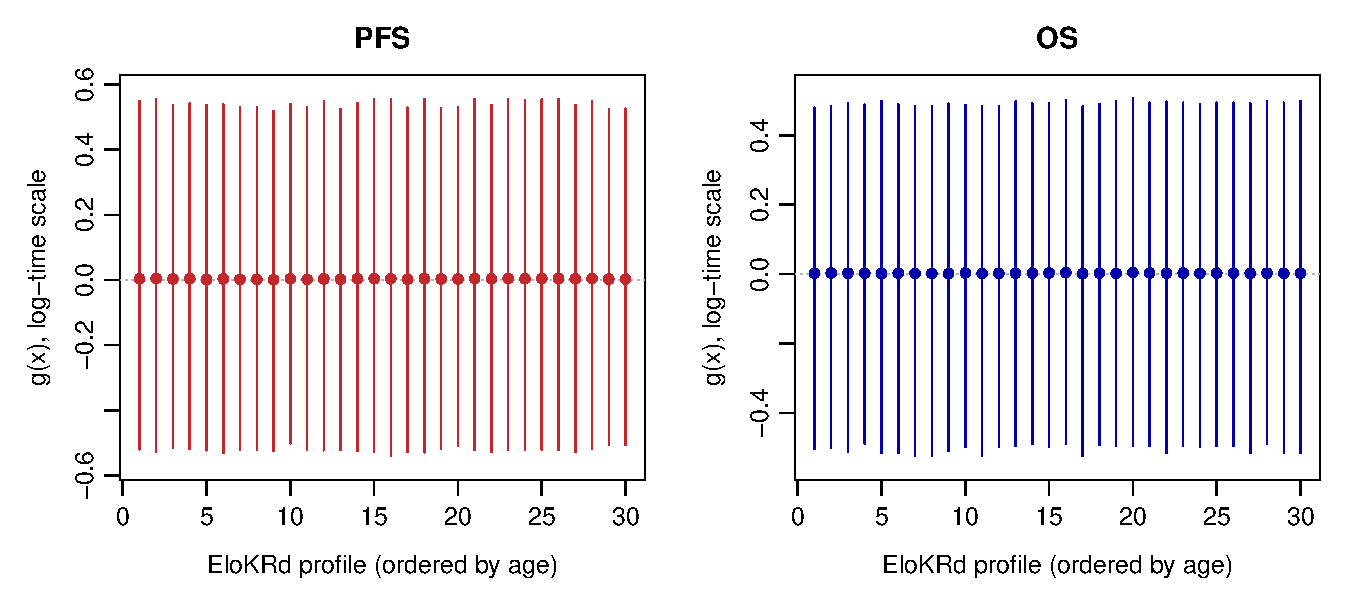
\includegraphics[width=\textwidth]{figures/fig_g_profiles.pdf}
\caption{Posterior mean and 95\% interval of the discrepancy $g(x)$ on the log-time scale at the 30 EloKRd profiles, ordered by age, at $N_{\rm target}=30$ for PFS (red) and OS (blue). In single-arm mode $g$ is a prior draw, so the intervals are centred at zero with SD $0.26$ everywhere; discrepancy uncertainty is therefore the same at every profile. Variation in external support is summarized by the local ESS map in Figure~\ref{fig:essmap}.}
\label{fig:gprofiles}
\end{figure}

\begin{figure}[htbp]
\centering
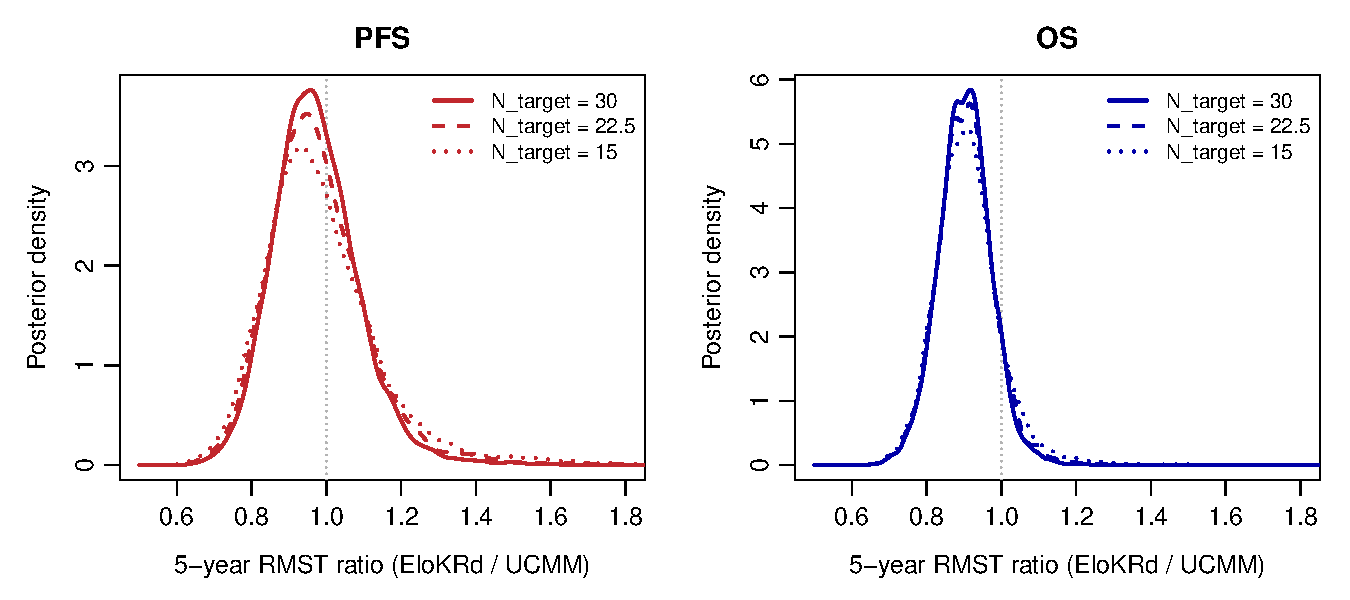
\includegraphics[width=\textwidth]{figures/fig_rmst_posterior.pdf}
\caption{Posterior density of the standardized 5-year RMST ratio for PFS and OS under LRC-BART at $N_{\rm target}=30$, $22.5$ and $15$ (harmonized coding, $H_f=10$, $w=1$).}
\label{fig:rmstpost}
\end{figure}

\subsection*{G.6 A conditional prior-cost comparison}

Consider a profile in a fixed region represented by one reached leaf in each of $H$ trees. Hold the partitions, weight $0<w<1$ and variances $0<\tau^2<\lambda^2$ fixed. For a specified configuration with $m$ slab leaves, let $u_h$ denote the $H$ discrepancy contributions and require $\sum_hu_h=\delta$. Relative to the all-spike density normalizers, each slab adds $c=\log\{w/(1-w)\}+\log(\lambda/\tau)$ to the negative log joint prior. The constrained minimum is
\[
Q_m(\delta)=mc+\min_{\sum_hu_h=\delta}\sum_h\frac{u_h^2}{2v_h}
=mc+\frac{\delta^2}{2S_m},\qquad
S_m=(H-m)\tau^2+m\lambda^2,\quad m\in\{0,\ldots,H\}.
\]
Here $v_h$ is the variance of contribution $h$. A Lagrange multiplier gives $u_h=\delta v_h/S_m$, so the remaining spike contributions participate in the optimum. If $c>0$, a specified configuration with $m\ge1$ has a smaller optimized cost than the all-spike configuration exactly when
\[
\delta^2>\frac{2mc}{(H\tau^2)^{-1}-S_m^{-1}}.
\]
The allowed values of $m$ are integers; minimizing over an unconstrained continuous value can give an infeasible allocation. If $c\le0$, the normalizing and weight penalty no longer favors the all-spike configuration even at zero discrepancy.

This calculation compares joint prior densities at constrained modes. Posterior indicator probabilities integrate over leaf parameters, sum over configurations and account for the likelihood and partition probabilities. They therefore do not follow from the ordering of $Q_m$. Nor does the calculation imply that a learned regional shift is assigned to one or two leaves. In a Gaussian common-mean comparison with regional sample sizes $n_1,n_2$ and a difference $\delta$ between source means, optimizing the pooled mean gives a negative log-likelihood loss of $\delta^2/[2(\sigma_1^2/n_1+\sigma_2^2/n_2)]$; its information is limited by the less precise source.

The separate ensemble in \eqref{eq:model} permits different partition and shrinkage priors for the external surface and its discrepancy. With fixed per-leaf spike variance, fewer discrepancy trees reduce the total spike variance at a profile. The slab range rule and the partitions also change with the model configuration, so this observation alone does not establish superior detection. The simulations assess the specified $H_g=5$ model, including the remaining regional surface loss.

\subsection*{G.7 The single-arm simulation in detail}

We provide further details of the single-arm study in Section~\ref{sec:sim_single}. The trial contributes $n_T$ treated subjects only, $200$ for Gaussian outcomes and $30$ or $200$ for survival outcomes, the $300$ RWD controls are the sole control source, and the estimands are standardized to the trial profiles. The comparators reduce to the complete-pooling models, the hierarchical models, BART-CP, and LRC-BART in the single-arm mode of Section~\ref{sec:singlearm} with $w=1$, at the absolute target $100$, at $0.9$ of the ceiling, and with the spike scale at the grid minimum, which is near-complete pooling of the leaf means; $w=0.9$ is the slab sensitivity. Sc3 is not identifiable without an internal control and is omitted. Table~\ref{tab:single} and Web Table~S6 report the results.

Under Sc1, BART-CP, the pooled LRC-BART and the target-$100$ LRC-BART have Gaussian RMSE $0.16$ with coverage $0.94$ to $1.00$, and at $n_T=30$ the survival RMST ratio has RMSE $0.16$ to $0.19$ with coverage $0.92$ to $0.97$.

Under Sc2, all methods have substantial bias. With the source assignment of Sc2 and no RCT controls, the RWD is the only information about the control surface at trial profiles that lie where RWD support is limited, and every method is far more biased than in the two-arm study: on the Gaussian ATE, LM-CP has bias $1.68$, BART-CP $0.41$ with coverage $0.75$, and LRC-BART $0.42$, and the survival median ratio at $n_T=30$ has biases of $0.8$ to $1.3$ for the tree models. Single-arm borrowing under measured confounding is a harder problem than the two-arm study, because no internal controls are available to reveal a discrepancy, and limited RWD overlap increases extrapolation; the rows reported for this scenario in the earlier version came from a different mechanism (Web Appendix~G.2).

For LRC-BART, uncertainty depends on the target relative to the ceiling. The single-arm ceiling is $27$ to $34$ in Sc2 and about $75$ at $n_T=30$ in Sc1, so an absolute target of $100$ is usually capped there. With $w=1$, the resulting small discrepancy scale approximates pooling. In Sc1 at $n_T=200$ the ceiling is about $160$, and target $100$ allows appreciable discrepancy uncertainty. The prior mean of a Gaussian control outcome or control log time remains centered on the external surface. Nonlinear survival-ratio means need not remain unchanged: under Sc1 with $n_T=200$, the median-ratio bias is $0.076$ for the pooled LRC-BART and $0.108$ for target $100$. The fractional target at $0.9$ of the ceiling widens intervals, with coverage $0.82$ to $0.99$ across the reported designs (Web Table~S6).

The $w=0.9$ sensitivity has posterior SD $1.4$ for the Gaussian ATE and $10$ to $34$ for the median ratio, with power $0$ and coverage $1$. Conditional on $w$ and the scales, the slab contributes $(1-w)H_g\tau_1^2$ to the pointwise prior variance of the counterfactual log-time mean. It can also change nonlinear ratio means substantially: under Sc1, the median-ratio bias at $n_T=200$ is $1.492$ with $w=0.9$, compared with $0.108$ with $w=1$. We therefore report $w=1$ for the primary single-arm analysis. HierLM and HierAFT with the stated hyperprior and no RCT controls draw the control surface from the hierarchy; their posterior SDs are $8$ for the Gaussian ATE and extremely large for the median ratio (Web Appendix~G.2).

\begin{center}
\scriptsize
\setlength{\tabcolsep}{3pt}
\renewcommand{\arraystretch}{0.8}
\begin{longtable}{llcccccccc}
\caption{Single-arm design, all methods, $R=500$. Columns as in Table~\ref{tab:single}; LRC-BART (100) and LRC-BART ($w=0.9$) use the absolute target 100, capped at the ceiling where infeasible, and LRC-BART (0.9, $w=0.9$) the fractional target with the slab.}\label{tab:single_full}\\
\toprule
& & \multicolumn{5}{c}{Treatment effect} & \multicolumn{2}{c}{Control} & \\
\cmidrule(lr){3-7}\cmidrule(lr){8-9}
Design & Method & Bias & SD & RMSE & Cov & Pow & Bias & RMSE & Prior ESS \\
\midrule
\endfirsthead
\multicolumn{10}{l}{\textit{Web Table S6, continued}}\\
\toprule
& & \multicolumn{5}{c}{Treatment effect} & \multicolumn{2}{c}{Control} & \\
\cmidrule(lr){3-7}\cmidrule(lr){8-9}
Design & Method & Bias & SD & RMSE & Cov & Pow & Bias & RMSE & Prior ESS \\
\midrule
\endhead
\midrule
\multicolumn{10}{r}{\textit{continued on the next page}}\\
\endfoot
\bottomrule
\endlastfoot
\multirow{8}{*}{\shortstack[l]{Gaussian, $n_T=200$\\ATE\\Sc1}} & LM-CP & 0.007 & 0.259 & 0.254 & 0.95 & 0.97 & $-$0.003 & 0.233 & --- \\
& HierLM & $-$0.014 & 8.239 & 0.497 & 1.00 & 0.00 & 0.018 & 0.487 & --- \\
& BART-CP & 0.010 & 0.163 & 0.162 & 0.94 & 1.00 & $-$0.003 & 0.127 & --- \\
& LRC-BART (pooled) & 0.007 & 0.165 & 0.162 & 0.94 & 1.00 & 0.001 & 0.127 & 172.3 \\
& LRC-BART (100) & 0.006 & 0.252 & 0.161 & 1.00 & 1.00 & 0.001 & 0.127 & 81.9 \\
& LRC-BART (0.9) & 0.007 & 0.202 & 0.163 & 0.98 & 1.00 & 0.000 & 0.128 & 115.8 \\
& LRC-BART ($w=0.9$) & 0.010 & 1.383 & 0.169 & 1.00 & 0.00 & $-$0.003 & 0.136 & 81.9 \\
& LRC-BART (0.9, $w=0.9$) & 0.006 & 1.372 & 0.169 & 1.00 & 0.00 & 0.001 & 0.133 & 116.4 \\
\midrule
\multirow{8}{*}{\shortstack[l]{Gaussian, $n_T=200$\\ATE\\Sc2}} & LM-CP & 1.682 & 0.417 & 1.734 & 0.01 & 1.00 & $-$1.676 & 1.726 & --- \\
& HierLM & 1.642 & 8.317 & 1.754 & 1.00 & 0.00 & $-$1.636 & 1.747 & --- \\
& BART-CP & 0.408 & 0.310 & 0.506 & 0.75 & 1.00 & $-$0.399 & 0.492 & --- \\
& LRC-BART (pooled) & 0.420 & 0.316 & 0.515 & 0.75 & 1.00 & $-$0.412 & 0.501 & 34.8 \\
& LRC-BART (100) & 0.421 & 0.316 & 0.515 & 0.76 & 1.00 & $-$0.413 & 0.501 & 34.7 \\
& LRC-BART (0.9) & 0.417 & 0.416 & 0.511 & 0.89 & 0.98 & $-$0.409 & 0.498 & 23.1 \\
& LRC-BART ($w=0.9$) & 0.416 & 1.329 & 0.511 & 1.00 & 0.00 & $-$0.408 & 0.498 & 34.8 \\
& LRC-BART (0.9, $w=0.9$) & 0.420 & 1.345 & 0.514 & 1.00 & 0.00 & $-$0.411 & 0.500 & 23.0 \\
\midrule
\multirow{8}{*}{\shortstack[l]{Survival, $n_T=30$\\median ratio\\Sc1}} & AFT-CP & 1.540 & 4.678 & 4.444 & 0.92 & 0.15 & $-$0.006 & 0.204 & --- \\
& HierAFT & $>\!10^{3}$ & $>\!10^{3}$ & $>\!10^{3}$ & 1.00 & 0.00 & $>\!10^{3}$ & $>\!10^{3}$ & --- \\
& BART-CP & $-$0.013 & 0.580 & 0.482 & 0.97 & 0.05 & $-$0.026 & 0.103 & --- \\
& LRC-BART (pooled) & 0.182 & 0.918 & 0.686 & 0.98 & 0.02 & $-$0.017 & 0.102 & 80.2 \\
& LRC-BART (100) & 0.180 & 0.917 & 0.686 & 0.98 & 0.03 & $-$0.017 & 0.099 & 79.0 \\
& LRC-BART (0.9) & 0.222 & 1.174 & 0.711 & 0.99 & 0.01 & $-$0.005 & 0.133 & 51.8 \\
& LRC-BART ($w=0.9$) & 1.423 & 11.199 & 1.959 & 1.00 & 0.00 & 0.318 & 0.433 & 79.3 \\
& LRC-BART (0.9, $w=0.9$) & 1.555 & 13.493 & 2.257 & 1.00 & 0.00 & 0.335 & 0.469 & 52.2 \\
\midrule
\multirow{8}{*}{\shortstack[l]{Survival, $n_T=30$\\median ratio\\Sc2}} & AFT-CP & 20.944 & 46.014 & 51.645 & 0.19 & 0.89 & $-$0.441 & 0.526 & --- \\
& HierAFT & $>\!10^{3}$ & $>\!10^{3}$ & $>\!10^{3}$ & 1.00 & 0.00 & $>\!10^{3}$ & $>\!10^{3}$ & --- \\
& BART-CP & 0.814 & 1.109 & 1.231 & 0.92 & 0.25 & $-$0.199 & 0.277 & --- \\
& LRC-BART (pooled) & 1.324 & 1.859 & 1.864 & 0.95 & 0.21 & $-$0.207 & 0.284 & 29.2 \\
& LRC-BART (100) & 1.329 & 1.865 & 1.875 & 0.95 & 0.20 & $-$0.208 & 0.284 & 29.1 \\
& LRC-BART (0.9) & 1.511 & 3.461 & 2.055 & 0.97 & 0.12 & $-$0.180 & 0.279 & 19.3 \\
& LRC-BART ($w=0.9$) & 4.243 & 28.669 & 5.305 & 1.00 & 0.00 & 0.179 & 0.537 & 28.9 \\
& LRC-BART (0.9, $w=0.9$) & 4.544 & 33.228 & 6.324 & 1.00 & 0.00 & 0.193 & 0.446 & 19.0 \\
\midrule
\multirow{8}{*}{\shortstack[l]{Survival, $n_T=30$\\RMST ratio\\Sc1}} & AFT-CP & 0.036 & 0.178 & 0.202 & 0.90 & 0.16 & 0.079 & 0.187 & --- \\
& HierAFT & $>\!10^{3}$ & $>\!10^{3}$ & $>\!10^{3}$ & 1.00 & 0.00 & 0.311 & 0.355 & --- \\
& BART-CP & $-$0.111 & 0.176 & 0.186 & 0.92 & 0.02 & $-$0.021 & 0.089 & --- \\
& LRC-BART (pooled) & $-$0.046 & 0.192 & 0.157 & 0.97 & 0.02 & 0.002 & 0.085 & 80.2 \\
& LRC-BART (100) & $-$0.046 & 0.192 & 0.157 & 0.97 & 0.02 & 0.002 & 0.084 & 79.0 \\
& LRC-BART (0.9) & $-$0.040 & 0.218 & 0.156 & 0.98 & 0.01 & 0.002 & 0.085 & 51.8 \\
& LRC-BART ($w=0.9$) & 0.080 & 0.998 & 0.200 & 1.00 & 0.00 & 0.020 & 0.089 & 79.3 \\
& LRC-BART (0.9, $w=0.9$) & 0.086 & 1.077 & 0.204 & 1.00 & 0.00 & 0.020 & 0.090 & 52.2 \\
\midrule
\multirow{8}{*}{\shortstack[l]{Survival, $n_T=30$\\RMST ratio\\Sc2}} & AFT-CP & 1.216 & 0.522 & 1.336 & 0.13 & 0.94 & $-$0.518 & 0.559 & --- \\
& HierAFT & $>\!10^{3}$ & $>\!10^{3}$ & $>\!10^{3}$ & 1.00 & 0.00 & 0.017 & 0.201 & --- \\
& BART-CP & 0.149 & 0.271 & 0.286 & 0.95 & 0.14 & $-$0.219 & 0.260 & --- \\
& LRC-BART (pooled) & 0.234 & 0.297 & 0.339 & 0.94 & 0.19 & $-$0.210 & 0.251 & 29.2 \\
& LRC-BART (100) & 0.235 & 0.297 & 0.340 & 0.94 & 0.19 & $-$0.211 & 0.251 & 29.1 \\
& LRC-BART (0.9) & 0.256 & 0.452 & 0.358 & 0.97 & 0.13 & $-$0.207 & 0.248 & 19.3 \\
& LRC-BART ($w=0.9$) & 0.527 & 2.689 & 0.643 & 1.00 & 0.00 & $-$0.185 & 0.228 & 28.9 \\
& LRC-BART (0.9, $w=0.9$) & 0.560 & 3.085 & 0.731 & 1.00 & 0.00 & $-$0.184 & 0.228 & 19.0 \\
\midrule
\multirow{8}{*}{\shortstack[l]{Survival, $n_T=200$\\median ratio\\Sc1}} & AFT-CP & 0.168 & 0.470 & 0.480 & 0.95 & 0.23 & 0.002 & 0.098 & --- \\
& HierAFT & $>\!10^{3}$ & $>\!10^{3}$ & $>\!10^{3}$ & 1.00 & 0.00 & $>\!10^{3}$ & $>\!10^{3}$ & --- \\
& BART-CP & 0.108 & 0.273 & 0.286 & 0.95 & 0.57 & $-$0.026 & 0.058 & --- \\
& LRC-BART (pooled) & 0.076 & 0.272 & 0.262 & 0.97 & 0.49 & $-$0.018 & 0.055 & 169.5 \\
& LRC-BART (100) & 0.108 & 0.565 & 0.284 & 1.00 & 0.17 & $-$0.008 & 0.055 & 81.7 \\
& LRC-BART (0.9) & 0.087 & 0.350 & 0.268 & 0.99 & 0.34 & $-$0.014 & 0.055 & 114.0 \\
& LRC-BART ($w=0.9$) & 1.492 & 15.408 & 4.227 & 1.00 & 0.00 & 0.318 & 0.402 & 81.8 \\
& LRC-BART (0.9, $w=0.9$) & 1.302 & 10.341 & 1.607 & 1.00 & 0.00 & 0.312 & 0.428 & 113.7 \\
\midrule
\multirow{8}{*}{\shortstack[l]{Survival, $n_T=200$\\median ratio\\Sc2}} & AFT-CP & 9.478 & 5.162 & 10.850 & 0.01 & 1.00 & $-$0.407 & 0.419 & --- \\
& HierAFT & $>\!10^{3}$ & $>\!10^{3}$ & $>\!10^{3}$ & 1.00 & 0.00 & $>\!10^{3}$ & $>\!10^{3}$ & --- \\
& BART-CP & 1.136 & 0.778 & 1.359 & 0.60 & 0.82 & $-$0.189 & 0.214 & --- \\
& LRC-BART (pooled) & 1.195 & 0.851 & 1.409 & 0.64 & 0.82 & $-$0.196 & 0.219 & 35.9 \\
& LRC-BART (100) & 1.193 & 0.856 & 1.410 & 0.65 & 0.81 & $-$0.196 & 0.219 & 35.9 \\
& LRC-BART (0.9) & 1.336 & 2.306 & 1.562 & 0.82 & 0.57 & $-$0.181 & 0.207 & 23.9 \\
& LRC-BART ($w=0.9$) & 3.935 & 26.373 & 4.611 & 1.00 & 0.00 & 0.142 & 0.396 & 36.2 \\
& LRC-BART (0.9, $w=0.9$) & 4.380 & 34.059 & 7.322 & 1.00 & 0.00 & 0.158 & 0.379 & 23.8 \\
\midrule
\multirow{8}{*}{\shortstack[l]{Survival, $n_T=200$\\RMST ratio\\Sc1}} & AFT-CP & $-$0.023 & 0.101 & 0.098 & 0.94 & 0.15 & 0.074 & 0.114 & --- \\
& HierAFT & $>\!10^{3}$ & $>\!10^{3}$ & $>\!10^{3}$ & 1.00 & 0.00 & 0.305 & 0.317 & --- \\
& BART-CP & $-$0.001 & 0.084 & 0.082 & 0.97 & 0.32 & $-$0.021 & 0.061 & --- \\
& LRC-BART (pooled) & $-$0.024 & 0.078 & 0.076 & 0.95 & 0.25 & 0.001 & 0.054 & 169.5 \\
& LRC-BART (100) & $-$0.020 & 0.121 & 0.076 & 0.99 & 0.09 & 0.003 & 0.054 & 81.7 \\
& LRC-BART (0.9) & $-$0.022 & 0.094 & 0.076 & 0.99 & 0.17 & 0.002 & 0.054 & 114.0 \\
& LRC-BART ($w=0.9$) & 0.109 & 1.179 & 0.275 & 1.00 & 0.00 & 0.021 & 0.057 & 81.8 \\
& LRC-BART (0.9, $w=0.9$) & 0.097 & 0.860 & 0.138 & 1.00 & 0.00 & 0.019 & 0.057 & 113.7 \\
\midrule
\multirow{8}{*}{\shortstack[l]{Survival, $n_T=200$\\RMST ratio\\Sc2}} & AFT-CP & 1.164 & 0.428 & 1.244 & 0.01 & 1.00 & $-$0.535 & 0.550 & --- \\
& HierAFT & $>\!10^{3}$ & $>\!10^{3}$ & $>\!10^{3}$ & 1.00 & 0.00 & 0.001 & 0.101 & --- \\
& BART-CP & 0.305 & 0.206 & 0.361 & 0.61 & 0.77 & $-$0.233 & 0.261 & --- \\
& LRC-BART (pooled) & 0.284 & 0.206 & 0.336 & 0.70 & 0.74 & $-$0.224 & 0.250 & 35.9 \\
& LRC-BART (100) & 0.284 & 0.207 & 0.336 & 0.69 & 0.73 & $-$0.224 & 0.250 & 35.9 \\
& LRC-BART (0.9) & 0.301 & 0.350 & 0.353 & 0.85 & 0.50 & $-$0.222 & 0.248 & 23.9 \\
& LRC-BART ($w=0.9$) & 0.562 & 2.419 & 0.633 & 1.00 & 0.00 & $-$0.200 & 0.228 & 36.2 \\
& LRC-BART (0.9, $w=0.9$) & 0.585 & 2.496 & 0.662 & 1.00 & 0.00 & $-$0.198 & 0.226 & 23.8 \\
\end{longtable}
\end{center}

